% $Id: hl.tex,v 1.3 1997/10/19 19:52:31 davek Exp davek $
\chapter{\candle: Modelling and Analysis in Practice}\label{chap:practice}
\section{Introduction}
This chapter presents \candle\ -- a {\bf CAN} {\bf D}evelopment 
{\bf L}anguage and {\bf E}nviron\-ment.
The purpose of \candle\ is to demonstrate
\begin{itemize}
\item a programming language for
distributed embedded systems whose components communicate using the 
CAN protocol, and
\item a development environment which integrates a variety of tools
  to support both system implementation and formal analysis.
\end{itemize} 

Our approach is very much influenced by \esterel~\cite{bg:92}, a
programming language and tool set for the construction and analysis of
uni-processor embedded systems. We aim to provide support for the view
that \bcandle\ offers an effective formal basis to support the \esterel\
philosophy of WYVIWYE (`What You Verify Is What You Execute') in the
case of CAN-based distributed systems. The emphasis in this chapter is
on the construction and analysis of models, rather than on code generation
and system implementation, which are mentioned only in connection with
model construction.
  
Work on \candle\ continues. Both the language and the development
environment are evolving. This chapter provides a snapshot of the
current status. The chapter is organised as follows. An informal
`tour' of the language, in the style of the \esterel\ Language
Primer~\cite{ber:98a}, is presented in~\Sec\ref{sec:prinformal} and a
simple data modelling language is introduced in~\Sec\ref{sec:prsdml}.
The translation to \bcandle\ is discussed in~\Sec\ref{sec:prtrans}.
Section~\ref{sec:prenv} outlines the main features of the development
environment which support the construction and analysis of formal
models of a \candle\ system.  A simple example is described
in~\Sec\ref{sec:prcanexample}.  Finally, conclusions and related work
appear in~\Sec\ref{sec:prconc}.

\section{A Tour of \candle\label{sec:prinformal}}
The \candle\ language is intended as a simple, high-level programming
language for use in the construction of distributed, CAN-based,
embedded systems. It can be used to describe the implementation of CAN
system designs, which may have been developed and explored at an
abstract level using \bcandle. Particular care has been taken to
ensure that a formal model of a system can be automatically extracted
from its \candle\ implementation. This has the benefits of removing
the task of model construction from the system developer and ensuring
that the model which is analysed is up to date with the current
implementation.  A \candle\ program can be translated automatically
into a program written in a \emph{host language}, such as C or Ada, in
order to construct a system implementation, or it can be translated
automatically into a \bcandle\ model, and thence to a Prolog or C
implementation of the corresponding labelled transition system, for
the purposes of simulation and verification. This section provides an
informal introduction to \candle. A complete grammar appears in
Appendix~\ref{chap:canparse} and details of the construction of a
formal model are given in \Sec\ref{sec:prtrans}.

\subsection{Modules}
A \candle\ program consists of a collection of \emph{modules}.  The
\candle\ module system is modelled on that of \esterel.  A module has a
name and, optionally, a declaration part and a body which is an
executable statement. One module is designated as the main program
module. Modules can use sub-modules by executing \emph{module
instantiation} statements. If module $A$ uses another module $B$, then
$A$ is said to \emph{depend} on $B$. The module dependency relation is
required to be acyclic, i.e. recursive module instantiation is prohibited.

Here is a simple example of a \candle\ module:
\begin{verbatim}
        module Flow is
          const 
            PERIOD : duration
          type
            flow_reading
          procedure
            ReadSensor(out flow_reading)
          channel
            k : (flow.flow_reading)
          var
            x : flow_reading
          behaviour
            every PERIOD do
              ReadSensor(x);
              snd(k,flow.x)
            end every
        end module
\end{verbatim}

The name of the module is {\tt Flow} and it implements the
behaviour of the flow sensor task described in~\Sec\ref{sec:bcexample}.
This is a task which periodically reads a flow sensor
and broadcasts its value on a communication channel. This behaviour is
shown in the module following the keyword {\tt behaviour}. The preceding 
sections are declarations of constants, types, procedures,
channels and variables. These language features are explained below.

\subsection{Data declarations}\label{ss:prdatadecls}
As with \esterel, \candle\ provides only a very limited facility for
describing data types and operations, instead it relies on an external
data language to provide the necessary definitions.  This approach
occasionally appears rather cumbersome but is extremely flexible in
practice. It provides portability, and more importantly, facilitates
the use of different languages for data modelling and
implementation. This allows the user to choose an abstract,
non-deterministic language, such as Z, for modelling, and a
traditional programming language, such as C or Ada, for
implementation.

A simple data modelling language, \sdml, is introduced later
in~\Sec\ref{sec:prsdml} in order to illustrate the use of an external
data language with \candle\ for the purpose of constructing system
models. With some additional work, more fully developed modelling
languages such as B~\cite{abr:96}, VDM~\cite{jon:90} and
Z~\cite{spi:88} could be used instead of \sdml. This would require the
reconcilation of different styles of semantic definition, e.g. the
denotational style of Z with the operational style of \bcandle. The
restriction of \candle\ to finite data types should simplify this problem
and future work will seek to exploit this benefit.

Data objects in \candle\ are either \emph{pre-defined} or
\emph{user-defined}. A few primitive data operations are provided in order 
to ease the expression of some typical idioms: assignment, comparison
and so on. All data objects are global to a program. Each data object
used within a module must be declared in that module. In the case that a 
data object is declared in several modules of a multi-module program,
it is required that the declarations are \emph{compatible} (see
\emph{module instantiation}~\Sec\ref{ss:prmodinst}).

\subsubsection{Types and Operators}
\candle\ provides the primitive types \trm{unit}, \trm{boolean},
\trm{\canMsgId} and \trm{duration}. 
\begin{itemize}
\item 
The \trm{unit} type contains the single value \trm{\unitval}.   
\item 
The \trm{boolean} type contains the constants \trm{true} and {\false}. 
The operations \trm{and}, \trm{or} and \trm{not} are defined. 
\item
The \trm{\canMsgId} type is the set of \emph{message identifiers}. For
any \candle\ program, \trm{\canMsgId} contains the message identifiers
occurring in the channel declarations of the program.
\item The \trm{duration} type is the set of time units for \candle\ 
programs. There are pre-defined functions \trm{Secs}, \trm{Msecs},
\trm{Usecs} and \trm{Cycles} which can be used to convert to the
\trm{duration} type an integer expression representing seconds, milliseconds, 
microseconds and clock cycles, respectively. For example, the
expression \trm{Msecs(30)} denotes the value of type \trm{duration}
which is equivalent to 30 milliseconds.
\end{itemize}
\candle\ allows the use of integer constants
{\tt 0, 1, -1, 2, -2, ...} and expressions involving the operators
\trm{+}, \trm{-}, \trm{*}, \trm{/} and \trm{mod}.  However, there is no
unbounded, primitive type \trm{integer}. It is assumed that integer
expressions evaluate to an element of some user-defined, finite
integer subrange. 

User-defined types are introduced into a \candle\ program simply by
declaring their names in a \emph{type declaration}, for example:
\begin{verbatim}
        type flow_reading
\end{verbatim}
Several type names can be introduced in a single type declaration, as
follows:
\begin{verbatim}
        type 
          byte;
          command; 
          resource_status  
\end{verbatim}
As has been mentioned, user-defined types are abstract, the concrete
definitions being given in an external data language.

The relational operators \trm{=}, \trm{/=}, \trm{<}, \trm{<=}, \trm{>=},
and \trm{>} can be used with any data type. If they are used, they must
be adequately defined in the external data language.

\subsubsection{Constants}
Constants are introduced by declaring their name and type, as follows:
\begin{verbatim}
        const N : byte
        const PERIOD : duration
\end{verbatim}
The value of a constant is defined either in the external data language or 
through module instantiation. There is no explicit constant value definition
in \candle.

\subsubsection{Variables}
Variables are assignable objects which have a name and a type. Variables
are declared with the \trm{var} declaration, as follows:
\begin{verbatim}
        var x : flow_reading
        var wl : water_level
\end{verbatim}
The variable declarations of a set of program modules give rise to a
single global state space. If a variable is declared
in two or more modules of a multi-module program then all declarations
must be type compatible. \candle\ inherits the notion of
type compatibility defined by the external
data language. 

A variable may be modified by assignments, procedure calls and message
receptions. It is not possible to assign a value to a variable in its
declaration. Each variable must be initialised explicitly by an 
executable statement before it is used. It is an error if any variable
is referenced by distinct behaviour expressions
occurring as the arguments of a parallel composition, i.e.
concurrently executing processes  cannot communicate via 
shared variables.

\subsubsection{Functions and Procedures}
Functions and procedures are introduced by declaring their names and
the type of their parameters. Parameters must be declared to have one
of the modes \trm{in}, \trm{out} or \trm{inout}, so that an
appropriate parameter-passing mechanism can be chosen for the host
language, for example: call-by-value for \trm{in} parameters and
call-by-reference for \trm{out} and \trm{inout} parameters. The
following example illustrates:

\begin{verbatim}
        procedure 
          ReadSensor(out flow_reading);
          UseResource()
        function 
          IsFullQueue(queue) : boolean
\end{verbatim}
If a parameter mode is not specified explicitly, the mode is assumed to be
\trm{in}. So the declaration of \trm{IsFullQueue} above is equivalent
to 
\[\trm{IsFullqueue(in queue): boolean}.\]
All parameters to a function must be \trm{in} parameters. Neither
procedures nor functions can have access to variables, other than
local variables, except through their parameter lists. It follows that
function evaluation in \candle\ is side-effect free.

\subsubsection{Channels}
Channels are the objects through which processes communicate by
passing messages.  Message passing is by broadcast using an abstracted
CAN protocol.  A message consists of a message identifier and an
optional data value.  A channel declaration introduces the name of a
channel and optionally a set of priority ordered message templates
which defines the messages which can be communicated by the
channel. For example,
\begin{verbatim}
    channel
      k : (ok.unit, node.command)
\end{verbatim}
declares a channel called \trm{k} which can transmit two kinds of messages: 
those consisting of the message identifier \trm{ok} and the unit value 
\trm{\unitval}, and those consisting of the message identifier \trm{node}
and any value of the type \trm{command}. The order of the message
templates is significant: higher priority messages are declared first.
So, for channel \trm{k}, \trm{ok} messages have higher priority than
\trm{node} messages.

In a multi-module program, the complete declaration of a channel is
derived from the (possibly partial) declarations of the channel in 
all modules where they occur. Not every declaration of a channel is required
to be complete in itself. A channel declaration is complete when
the identifier, priority ordering and value type of every message
mentioned in the program body can be determined. Multiple channel
declarations must be compatible, which means that they must agree on
the priority ordering and value type of all messages.
\label{page:prchannelcompat} For example, the
following are compatible declarations of the channel \trm{k} declared
above:
\begin{verbatim}
    channel k              -- declare the name only
    channel k : (ok.unit)  -- not all message templates declared
    channel k : (ok, node) -- message types not yet specified
\end{verbatim}
Whereas these declarations are not compatible:
\begin{verbatim}
    channel k : (node.command, ok.unit) -- wrong priority ordering
    channel k : (node.unit)             -- incompatible type
\end{verbatim}
    
\subsubsection{Exceptions}
\candle\ allows exceptions to be declared and used in 
\trm{trap} and \trm{exit} statements. An exception has a
name and can carry a value. An exception is declared like a variable,
by giving its name and the type of value carried:
\begin{verbatim}
        exception SensorFailure : unit
        exception Alarm : alarm_t
\end{verbatim}
As with variables, exceptions form part of the global state space of a
program. If an exception is declared in two or more modules of a
multi-module program, the declarations must be type compatible.

\subsection{Expressions}
The expression language of \candle\ is very simple. It is built from:
\begin{itemize}
\item constant values of the predefined types \trm{unit}, \trm{boolean},
  \trm{\canMsgId} and \trm{duration}, together with the integer constants 
  from some finite integer subrange;
\item variable identifiers;
\item a small number of built-in operators, including: \trm{and}, \trm{or},
  \trm{not}, \trm{+}, \trm{-}, \trm{*}, \trm{/}, \trm{mod}, \trm{=},
  \trm{/=}, \trm{<}, \trm{<=}, \trm{>=} and \trm{>};
\item the pre-defined functions \trm{Secs}, \trm{Msecs}, \trm{Usecs}
  and \trm{Cycles};
\item the exception value operator \trm{?}, which returns the value
  bound to a named exception;
\item user-declared function calls.
\end{itemize}
Here are some examples of \candle\ expressions:
\begin{verbatim}
        temperature > maxTemperature
        count mod N = 0 or count < 10
        Alarm2String(?Alarm)
        Usecs(30)
\end{verbatim}
\candle\ adopts the type compatibility rules of the external data language.
  
\subsection{Statements}
\subsubsection{\trm{null} and \trm{idle} statements}
The simplest \candle\ statements are \trm{null} and \trm{idle}.
Execution of the \trm{null} statement terminates instantaneously with no 
effect on the state of the network or data environment.
Execution of the \trm{idle} statement similarly leaves the program context
unchanged but delays forever without terminating.
 
\subsubsection{Send and Receive statements}
Broadcast message transmission is initiated by the
\trm{snd} statement, as follows:
\begin{verbatim}
        snd(k, node.req)
        snd(k, ok)
\end{verbatim}
The first parameter names the communication channel on which the message
is to be transmitted. The second parameter consists of a message identifier
and, optionally, a data value, which together constitute the message
to be transmitted, e.g. \trm{node.req} where \trm{node} is
the message identifier and \trm{req} is the data value. In the case that
no data value is given, the unit value is assumed, e.g. \trm{snd(k, ok)}
is equivalent to \trm{snd(k, ok.\unitval)}. The \trm{snd} statement
is non-blocking.

Willingness to receive a broadcast message is indicated by the
\trm{rcv} statement, as follows:
\begin{verbatim}
        rcv(k, node.x)
        rcv(k, ok)
\end{verbatim}
The first parameter names the communication channel from which the
message is to be received. The second parameter gives the required
message identifier and, optionally, the data variable to which the
received data value is to be assigned, e.g.  \trm{rcv(k, node.x)}
can receive a message having the identifier \trm{node} and will
assign the data value of the message to the variable \trm{x}.
In the case that a message carries the unit data value, it is not
necessary to specify a data variable to receive it, e.g. 
\trm{rcv(k, ok)} succeeds when an \trm{ok} message is
available on channel \trm{k}. 

The \trm{rcv} statement is blocking -- if there is no suitable message
available, the calling process waits.

\subsubsection{Elapse statement}
The \trm{elapse} statement is used to cause a process to wait for a
specified period of time.
\begin{verbatim}
        elapse Secs(5)
        elapse Msecs(10)
        elapse Cycles(50) 
\end{verbatim} 
The constant expression denoting the extent of the delay is required to be
evaluable at compile-time and must be of type \trm{duration}. 

It is assumed that a compiler will generate code for the \trm{elapse}
statement which, starting from the initiation of its execution,
will produce a delay which is as close as possible to the requested value.
Construction of the model of the \trm{elapse} statement needs to
take into account how the generated code and the run-time
environment operate in creating the delay. This is discussed in more detail
in~\Sec\ref{sec:prtrans}.

\subsubsection{Assignment and Procedure Call}
The assignment statement has the form 
\begin{zed}
\t2 x \trm{ := } e
\end{zed}
where $x$ is a variable and $e$ is a data expression. The variable
and the expression must be type compatible. The bounds on the time taken
to execute an assignment statement for a given variable type are determined
either by analysis of the code which is generated to perform the assignment, 
or by an explicit \trm{bounds} declaration in the external data model,
as discussed in~\Sec\ref{sec:prsdml}.

A procedure call has the form
\begin{zed}
\t2  P(e_1, e_2 ,..., e_n)
\end{zed}
where $e_1$ \ldots $e_n$ are data expressions, whose mode and
type are compatible with the corresponding parameters in the
declaration of the procedure $P$. Bounds on the procedure execution
time are determined as for the assignment statement.

\subsubsection{Sequential and Parallel statements}
\candle\ allows statements to be combined both in \emph{sequence} and
in \emph{parallel}. The sequencing of behaviours is described
by the sequential composition operator ``\trm{;}'', e.g.
\begin{verbatim}
    ReadSensor(x) ; snd(k,flow.x)
\end{verbatim} 
where execution of the procedure \trm{ReadSensor} is immediately followed
by execution of the communication statement \trm{snd(k,flow.x)}.

In the behaviour
\begin{zed}
\t2 s_1 \sq s_2
\end{zed}
the statement $s_1$ is started as soon as the sequence is started.
If $s_1$ terminates, then $s_2$ is started at once. If $s_1$ does not
terminate, then $s_2$ is never started.

The \emph{parallel} statement is written using the parallel composition
operator ``\trm{|}'', e.g.
\begin{verbatim}
    ReadSensor(x) ; snd(k,flow.x) | rcv(k,flow.y) ; AdjustValve(y)
\end{verbatim}
The parallel composition operator has lower precedence than sequential
composition. It is only allowed at the top-level of a behaviour.

In the behaviour
\begin{zed}
\t2 s_1 \parallel s_2
\end{zed}
the statements $s_1$ and $s_2$ are both started as soon as the parallel
behaviour is started, and are assumed to execute concurrently. The
parallel behaviour terminates when both $s_1$ and $s_2$ terminate.
Parallel composition in \candle\ is asynchronous and communication is
restricted to message passing via broadcast channels. In order to 
guard against interference between the behaviours $s_1$ and $s_2$, it is
required that the sets of variables and exceptions to which they refer are
disjoint.

\subsubsection{If statement}
The \trm{if} statement is used to allow the execution of a program to 
depend upon the value of boolean data expressions. The general form of an
\trm{if} statement is
\begin{zed}
\t2    \trm{if } e_0 \trm{ then } s_0 \\
\t2    \trm{elsif } e_1 \trm{ then } s_1 \\
\t2    \vdots \\
\t2    \trm{elsif } e_n \trm{ then } s_n \\
\t2    \trm{else } s \\
\t2    \trm{end if}
\end{zed}
where $e_0$ to $e_n$ are boolean expressions and $s_0$ to
$s_n$ are statements, as is $s$. The \trm{elsif} and \trm{else}
parts of the statement are optional.  The expressions $e_0$ to
$e_n$ are evaluated in sequence. The first $\True$ expression
causes the corresponding statement to be executed. If
none of the expressions evaluates to $\True$, then the \trm{else}
statement $s$ is executed if it is present, otherwise the
\trm{if} statement terminates. 

\subsubsection{Iteration statements}
Repetitive behaviours can be described in \candle\ using a variety
of iteration constructs. The simplest iteration construct is the 
basic \trm{loop} statement which allows the expression of a behaviour
which is executed repeatedly forever. The \emph{named} \trm{loop}
statement extends the basic loop by providing a \emph{name} which can
be used in an \trm{exit} statement to cause the named loop to be terminated.
The \trm{every} statement allows the description of a behaviour which is
executed \emph{periodically}.

A \emph{basic} loop statement has the form
\begin{zed}
\t2     \trm{loop do} \\
\t3          s \\
\t2     \trm{end loop} 
\end{zed}
where $s$ is a statement. A basic loop executes the statement $s$
repeatedly forever.

Here is an example of the use of a basic
loop in implementing the \trm{Valve} process for the flow regulator
example of~\Sec\ref{sec:bcexample}: 
\begin{verbatim}
        module Valve is
          type
            flow_reading
          procedure
            AdjustValve(flow_reading)
          channel
            k : (flow.flow_reading)
          var
            x : flow_reading
          behaviour
            loop do
              rcv(k,flow.x);
              AdjustValve(x)
            end loop
        end module
\end{verbatim}
The process repeatedly waits to receive a $flow$ message and then
adjusts a valve accordingly.

A \emph{named} loop statement has the form
\begin{zed}  
\t2     \trm{loop } LoopName \trm{ do} \\
\t3          s \\
\t2     \trm{end loop}
\end{zed}
where $s$ is a statement and $LoopName$ is an identifier. 

In the case of a named loop, an \trm{exit}
statement, occurring as part of the statement $s$, causes the loop
to be terminated, e.g.
\begin{verbatim}
        x := 0;
        loop Transmit do
          snd(k, value.x);
          x := x + 1;
          if x = 10 then exit Transmit end if
        end loop
\end{verbatim}
The \trm{Transmit} loop is terminated after ten iterations.

Another form of repetition is introduced in \candle\ by the 
\trm{every} statement, which has the form:
\begin{zed}
\t2 \trm{every } T \trm{ do} \\
\t3       s \\
\t2  \trm{end every}
\end{zed}
where $T$ is a statically evaluable constant expression of
type \trm{duration} and $s$ is a statement. The \trm{every}
statement causes $s$ to be executed periodically, with execution
beginning every $T$ time units. For example,
\begin{verbatim}
      every Msecs(10) do
         ReadSensor(x);
         snd(k, flow.x)
      end every
\end{verbatim}
causes execution of the statement body to be initiated immediately and
to be executed periodically every $10$ msecs thereafter.

\subsubsection{Select statement}
A basic \trm{select} statement allows a choice to be made from several
alternative statements, depending on the reception of a message or the
elapse of a time delay. It has the general form:
\begin{zed}
\t2 \trm{select} \\
\t3 \trm{:: rcv}(k_1, i_1.x_1) \sq s_1 \\
\t3 \trm{:: rcv}(k_2, i_2.x_2) \sq s_2 \\
\t3 \vdots \\
\t3 \trm{:: rcv}(k_n, i_n.x_n) \sq s_n \\
\t3 \trm{:: elapse} T \sq s \\
\t2 \trm{end select}
\end{zed}
If one of the \trm{rcv}$(k_j, i_j.x_j)$ statements succeeds, then the
program continues by executing the statement $s_j$. If more than 
one of the \trm{rcv} statements can succeed simultaneously, then a choice 
between them is made non-deterministically. If no \trm{rcv} statement can 
succeed before $T$ time units have elapsed, then statement $s$ is 
executed.

\candle\ also offers an extended \trm{select} statement, which has the form
\begin{zed}
\t2 \trm{select} \\
\t3 \trm{:: rcv}(k_1, i_1.x_1) \sq s_1 \\
\t3 \trm{:: rcv}(k_2, i_2.x_2) \sq s_2 \\
\t3 \vdots \\
\t3 \trm{:: rcv}(k_n, i_n.x_n) \sq s_n \\
\t3 \trm{:: elapse} T \sq s \\
\t2 \trm{in} \\
\t3 body \\
\t2 \trm{end select}
\end{zed}
and behaves like a basic select statement, except that the statement
$body$ is executed while a message reception or timeout is
awaited. If a message is received or the time delay elapses before
$body$ terminates, then the execution of $body$ is aborted and
execution of the corresponding statement is started. If $body$
terminates before a message is received or the time delay elapses then
the \trm{select} statement terminates.

\pagebreak\noindent
The following example illustrates both forms of the \trm{select}
statement:
\begin{verbatim}
        select  
          :: rcv(k,shutdown); ShutDown(); idle
        in
          loop do
            select
              :: rcv(k,pump_on) ; PumpOn()
              :: rcv(k,pump_off) ; PumpOff()
            end select
          end loop
        end select
\end{verbatim}
The body of the outer \trm{select} statement is a \trm{loop} which
repeatedly waits for either a \trm{pump_on} or \trm{pump_off} message
and then executes the appropriate procedure. However, if a \trm{shutdown}
message is received, the \trm{loop} is aborted, the \trm{ShutDown} 
procedure is executed and the process idles.
 
\subsubsection{Trap and Exit statements}
The \trm{trap} statement can be used to trap exceptions raised in a
program block and to define an appropriate behaviour for handling each
trapped exception. The \trm{trap} statement has the general form:
\begin{zed}
\t2 \trm{trap} \\
\t3 \trm{:: } x_1 \trm{ => } s_1 \\
\t3 \trm{:: } x_2 \trm{ => } s_2 \\
\t3 \vdots \\
\t3 \trm{:: } x_n \trm{ => } s_n \\
\t2 \trm{in} \\ 
\t3    body \\
\t2 \trm{end trap}
\end{zed}
where each $x_i$ is a previously declared exception identifier and
each $s_i$ is a statement which acts as the handler for exception
$x_i$. Execution of the \trm{trap} statement begins by executing
the statement $body$. An exception can be raised in 
$body$ by using the \trm{exit} statement. If an exception is
raised, the execution of $body$ is aborted and, if the exception is
trapped, execution of the exception handler is started. In the case of
a valued exception, the \trm{exit} statement is used to define the
value of the exception, e.g.
\begin{verbatim}
        exit Alarm(flowHigh)
\end{verbatim}
raises the \trm{Alarm} exception and binds to it the value
\trm{flowHigh}. Notice that the value of an exception can be
referred to in its handler by using the \trm{?} operator, as in
\begin{zed}
\t2 \trm{trap} \\
\t3 \vdots \\          
\t3 \trm{:: Alarm => if ?Alarm = flowHigh then ... end if} \\
\t3 \vdots \\          
\t2 \trm{in} \\
\t3 \vdots \\          
\t3 \trm{exit Alarm(flowHigh);} \\
\t3 \vdots \\          
\t2 \trm{end trap}
\end{zed}
It is an error to attempt to refer to the value of an
exception outside its handler.

\subsubsection{Module Instantiation\label{ss:prmodinst}}
A module can be instantiated within another module by using a module 
instantiation statement. This has the forms
\[
\begin{array}{ll}
M & \trm{-- module identifier, no renaming} \\
M \trm{[}R\trm{]}  & \trm{-- module identifier, with renaming}
\end{array}
\]
where $M$ is the name of a module and $R$ is a list of 
renamings. The instantiation is syntactically replaced by the body
of the module $M$ renamed according to $R$. A renaming
$e / I$ causes all occurrences of the identifier $I$ in 
$M$ to be replaced with the expression $e$. This is
simple textual replacement; $e$ is not evaluated at this point.
The resulting module must be well-formed. 

All declarations are global to a \candle\ program. Therefore, the
declarations of the instantiated module are exported to the parent
module. If the parent and child modules both declare objects having the
same name, then the declarations must be compatible. Compatibility
for constants, variables, procedures and functions is simply
type compatibility as defined by the external data language. Compatibility
for channels is described in~\Sec\ref{ss:prdatadecls} 
page~\pageref{page:prchannelcompat}. 

Here is an example of the use of module instantiation, which uses the
\trm{Flow} and \trm{Valve} modules declared earlier.  
\begin{verbatim}
        module FlowRegulator is
          behaviour
            Flow[Msecs(10)/PERIOD] | Valve[y/x]    
        end module
\end{verbatim}
The details for the expansion of a module instantiation
are as given below.

Firstly, a module is called \emph{independent} if it does not contain any
module instantiation statements in its body; otherwise it is 
said to be \emph{dependent}.
 \begin{itemize}
\item
To expand an independent module instantiation $M1[R]$ in a parent module $M$:
\begin{enumerate}
\item Apply the renaming $R$ to $M1$, giving the renamed module
  $M1'$. 
\item Textually replace the module instantiation statement with the body of 
  the module $M1'$.
\item Merge the declarations of $M1'$ with the 
  declarations of its parent module $M$.
\end{enumerate}
\item
To expand a dependent module instantiation $M1[R]$ in a parent module 
$M$:
\begin{enumerate}
\item Recursively expand any module instantiations in the body of $M1$.
\item Expand the remaining independent module instantiation in $M$, as 
  described above. 
\end{enumerate}
\end{itemize}

The effect of applying these rules in expanding the instantiations in the
module \trm{FlowRegulator} is shown in the module
\trm{FlowRegulator\_E} of Figure~\ref{fig:prmodinstex}.
\begin{figure}
\begin{center}
\begin{minipage}{.8\linewidth}
\small
\begin{verbatim}
        module FlowRegulator_E is
          type
            flow_reading
          procedure
            ReadSensor(out flow_reading);
            AdjustValve(flow_reading)
          channel
            k : (flow.flow_reading)
          var
            x : flow_reading;
            y : flow_reading
          behaviour 
            every Msecs(10) do
              ReadSensor(x);
              snd(k,flow.x)
            end every
          | 
            loop do
              rcv(k,flow.y);
              AdjustValve(y)
            end loop
        end module
\end{verbatim}
\end{minipage}
\end{center}
\caption{Flow Regulator: Instantiated and Renamed \label{fig:prmodinstex}}
\end{figure}
 
\section{\sdml: Simple Data Modelling Language\label{sec:prsdml}}
We require an external data language in order to provide complete examples of
the modelling of systems using \candle. It is outside the scope of this thesis
to discuss the connection of \candle\ to a standard data language such
as Z. Instead, we introduce a simple data modelling language, \sdml,
which is an extension of Dijkstra's non-deterministic language of 
guarded commands~\cite{dij:76}. A \sdml\ program is just a sequence of type, 
constant, function and procedure declarations.  
This section gives an informal introduction to \sdml. A complete grammar is 
given in Appendix~\ref{chap:datparse}.  
\subsection{Types}
\sdml\ has the same pre-defined types as \candle: \trm{unit},
\trm{boolean}, \trm{id} and \trm{duration}. In addition, the 
following types can be constructed:
\begin{itemize}
\item \emph{enumeration} types, which are declared by enclosing
  between braces a comma-separated list of the values of the type,
  e.g. \verb'{low, ok, high}';
\item \emph{subrange} types, which have the form $low$ \trm{..} $high$, where 
  $low$ and $high$ are expressions which are evaluable at 
  compile-time and denote values of some ordered type; values of 
  the subrange type are all those of the underlying ordered type from $low$ 
  to $high$ inclusive, e.g. \trm{0..4} defines the values 
  \trm{0,1,2,3} and \trm{4};
\item \emph{record} types, which are are tuples of named elements, enclosed 
  by the delimiters \verb'{|' and \verb'|}', e.g. \\
  \verb'      {| numerator : 0..9999; denominator : 0..9999 |}' \\
  consists of a pair of integers in the range \trm{0..9999};
\item \emph{array} types, which are sequences of values of
  some previously defined type, indexed by a subrange of some ordered
  type, e.g. \trm{array 0..4 of boolean}.  
\end{itemize}
A type can be given a name in a type declaration, as follows:
\begin{verbatim}
        type flow_reading is unit 
        type water_level is {low, ok, high}
        type byte is 0..255
        type rational is {| numerator   : 0..9999; 
                            denominator : 0..9999 |};
             byte_array is array 0..3 of byte
\end{verbatim}
Recursive type declarations are not allowed.

In modelling the data of a system, it is usually the case that we
abstract from the full set of data values of the underlying
implementation and use a smaller set of values which is large
enough to preserve the system properties of interest. For example, in
the declaration of \trm{flow\_reading} above, we have abstracted
entirely from the set of flow readings and use the
\trm{unit} type instead. However, in order to calculate the
communication latency of messages which contain
\trm{flow\_reading} data, it is necessary to know the size of its
representation as implemented.  We extend type declarations to allow
this information to be included:
\begin{verbatim}
        type flow_reading is unit size Bytes(4)
\end{verbatim}
where the \trm{size} clause introduces an expression giving the size
of the implemented data representation of the type. The pre-defined
functions \trm{Bytes} and \trm{Bits} can be used in \trm{size} expressions. 

\subsection{Constants}
Constants are declared using the keyword \trm{const}:
\begin{verbatim}
        const
          req             : command;
          NUMBER_OF_NODES : 0..255 is 10;
          MAX_TEMPERATURE : 0..65535 is 25000
\end{verbatim}
where each constant is declared by giving its name, its type and, optionally,
its value. The value of a constant is given by an expression following
the keyword \trm{is}, as in \\
\verb'      const NUMBER_OF_NODES : 0..255 is 10'. \\
An expression used in a constant definition must be evaluable at compile-time.

\subsection{Expressions}
Expressions in \sdml\ are the same as in \candle, with the following 
extensions:
\begin{itemize}
\item The pre-defined functions \trm{Bytes} and \trm{Bits} are provided
  for use in \trm{size} declarations.
\item The \emph{non-deterministic} expression \trm{any} type\emph{Identifier},
  evaluates to any one of the values of the type
  denoted by type\emph{Identifier}. For example, the expression 
  \trm{any water_level} evaluates to any one of \trm{low}, \trm{ok} or 
  \trm{high}. The use of the \trm{any} expression is restricted to simple 
  assignment, e.g. \\ \trm{wl} \trm{:=} \trm{any water_level}.   
\item A \emph{field selector} expression has the form $x$\trm{.}$f$, where
  \trm{x} is a record variable and $f$ is a field.
  For example, if \trm{x} is a record variable whose value is
  \verb'{| numerator = 1; denominator = 2 |}', then
  the value of \verb'x.numerator' is \trm{1} and the value of
  \verb'x.denominator' is \trm{2}.  
\item An \emph{array element selector} expression has the form
  $a\trm{[}i\trm{]}$, where $a$ is an array variable and $i$ is an
  expression denoting a value of the index type of $a$. For
  example, if \trm{a} is an array variable whose value is
  \verb'[| 0; 2; 4; 8 |]', then \verb'a[2]' is an expression whose value is 
  \trm{4}, assuming that the index type of \verb'a' is \verb'0..3'.
\end{itemize}

\subsection{Functions and Procedures}
Function and procedure declarations consist of a \emph{header}, which has 
the same syntax as in \candle\, and a \emph{body} which is written after
the keyword \trm{is}:
\begin{verbatim}
        function IsEmptyQueue(q : queue) : boolean is
          bounds Cycles(30) ; Cycles(45)
          begin
            return (q.rear = 0)
          end
        
        procedure Swap(inout x : byte; inout y : byte) is
          bounds Usecs(100) ; Usecs(125)
          var temp : byte
          begin
            temp := x;
            x := y;
            y := temp
          end
\end{verbatim}
The body of the function or procedure consists of a \emph{bounds}
declaration, a \emph{local variable} declaration and a \emph{statement}.
The bounds declaration allows the user to state
lower and upper bounds on the execution time of the function or procedure.
In the declaration 
\begin{verbatim}
      bounds Cycles(30) ; Cycles(45)
\end{verbatim}
the lower (resp. upper) bound is \trm{30} (resp. 45) clock
cycles.  The expression for each bound must be of type
\trm{duration}. It is usual to state bounds in clock cycles and
to allow a \trm{duration} value to be calculated automatically when
the execution environment is fixed for a particular invocation of the
sub-program. However, it is possible to state bounds which are
independent of the execution environment, as in the declaration of
\trm{Swap}. In the declaration
\trm{bounds} $\tlb$ \trm{;} $\tub$, it is required that $\tlb \leq \tub$. 
The `infinite bound' $\infinity$ can be used and is written as \trm{\~{}},
e.g. \verb'bounds Cycles(30); ~'. 

A function declaration is required to respect the following constraints:
\begin{itemize}
\item the non-deterministic assignment statement is not allowed in 
  a function body, nor in the body of any procedure which is called by
  a function;
\item all function parameters are required to have the mode \trm{in};
\item the only variables which can be referred to in the body of a function
  are actual parameters and local variables.
\end{itemize}

\subsection{Statements}
A \sdml\ statement is either an atomic statement or a sequential
statement. The atomic statements are:
\begin{itemize}
\item the \trm{skip} statement which terminates leaving the data state 
  unchanged;
\item the assignment statement $x \trm{ := } e$ which causes the value of
  the expression $e$ to be bound to the variable $x$;
\item the procedure call statement $P(e_1,\ldots e_n)$, where $P$
  is the name of a procedure and $e_1$ to $e_n$ are the actual 
  parameters;
\item the return statement $\trm{return } e$ which is used in a function
  body to indicate that the value of the function is $e$;
\item the non-deterministic \trm{if} statement
  \begin{zed}
    \t2  \trm{if} \\
    \t3  \trm{:: } e_1 \trm{ => } s_1 \\
    \t3  \trm{:: } e_2 \trm{ => } s_2 \\
    \t3 \vdots \\
    \t3  \trm{:: } e_n \trm{ => } s_n \\
    \t2  \trm{fi}
  \end{zed}
  where each $e_i$ is a boolean expression, called a \emph{guard}, 
  and each $s_i$ is a statement which can be chosen for execution if
  the associated guard evaluates to $\True$. When more than one guard is 
  $\True$, the statement to be executed is chosen non-deterministically
  from among the statements whose guards are $\True$. It is required
  that at least one of the guards in an \trm{if} statement is $\True$.
\item the non-deterministic \trm{do} statement 
  \begin{zed}
    \t2 \trm{do} \\
    \t3  \trm{:: } e_1 \trm{ => } s_1 \\
    \t3  \trm{:: } e_2 \trm{ => } s_2 \\
    \t3 \vdots \\
    \t3  \trm{:: } e_n \trm{ => } s_n \\
    \t2 \trm{od}
  \end{zed}
  whose branches are as for the \trm{if} statement. If some guard 
  evaluates to $\True$, a statement is chosen for execution and the \trm{do}
  statement is repeated. The \trm{do} statement terminates when no
  guard evaluates to $\True$. The user is required to
  establish the termination of every \trm{do} statement in a
  \sdml\ program. 
\end{itemize}
In a sequential statement $s_1 \trm{ ; } s_2$, the statement $s_1$
is executed and, when the execution of $s_1$ terminates, execution
of $s_2$ begins.

\subsection{Semantics}\label{ss:prsdmlsemantics}
\sdml\ is a block-structured, statically-scoped,
sequential programming language. It introduces a few familiar
mechanisms for declaring types, constants, functions and
procedures. Statements are essentially as in Dijkstra's
guarded command language~\cite{dij:76}. We assume the existence of a
semantic function which gives the meaning of \sdml\ statements. This
function is required later in constructing a \bcandle\ model from a
\candle\ program where \sdml\ is used as the external data language.

Let $\canSmnt$ be the set of \sdml\ statements.  For a \sdml\ program,
let $\Var$ be the set of data variables and $\V$ be the set of data
values. Let $\valuation \defs \Var \fun \V$ be the set of
valuations. Then, the semantic function 
\[ \evalCanSmntFN : \canSmnt \fun \valuation \fun 2^\valuation \]
gives the meaning of \sdml\ statements, where $\evalCanSmnt{s}\val$
denotes the set of valuations which are possible results of executing
the statement $s$ under the valuation $\val$.

Notice that because \sdml\ is a non-deterministic language, a
statement maps a valuation to a \emph{set} of result valuations.
Nevertheless, the definition of the semantic function is quite
straightforward; the interested reader is referred to standard texts
such as Schmidt~\cite{sch:86} or Winskel~\cite{win:93} for further
details.
   
\section{Constructing a Formal Model\label{sec:prtrans}}
This section describes how a \candle\ program can be translated into
\bcandle, so that its behaviour can be simulated or verified. The
construction of a \bcandle\ model, which conservatively approximates
the implemented system, depends not only on the \candle\ program but
also on features of the code generator and the execution
environment.  It is outside the scope of this thesis to discuss these
aspects fully.  The intention here is to provide a general
framework for the translation, which can be adapted to accommodate
particular requirements.

It is assumed, without loss of generality, that
a \bcandle\ model is constructed from a single \candle\ 
module of the form:
\begin{zed}
\trm{module } moduleName \trm{ is} \\
\t1 \trm{type } typeDecl_1; \ldots ; typeDecl_n \\
\t1 \trm{const } constantDecl_1; \ldots ; constantDecl_n \\
\t1 \trm{var } variableDecl_1; \ldots ; variableDecl_n \\
\t1 \trm{function } functionDecl_1 ; \ldots ; functionDecl_n \\
\t1 \trm{procedure } procedureDecl_1 ; \ldots ; procedureDecl_n \\
\t1 \trm{channel } channelDecl_1 ; \ldots ; channelDecl_n \\
\t1 \trm{exception } exceptionDecl_1 ; \ldots ; exceptionDecl_n \\
\t1 \trm{behaviour } statement \\
\trm{end module}
\end{zed}
and a single \sdml\ module of the form:
\begin{zed}
\trm{data } moduleName \trm{ is} \\
\t1 \trm{type } typeDecl_1; \ldots ; typeDecl_n \\
\t1 \trm{const } constantDecl_1; \ldots ; constantDecl_n \\
\t1 \trm{function } functionDecl_1 ; \ldots ; functionDecl_n \\
\t1 \trm{procedure } procedureDecl_1 ; \ldots ; procedureDecl_n \\
\trm{end data}
\end{zed}
That is to say, module instantiation statements are expanded, and
declarations are collected, to give a well-formed, stand-alone
\candle\ module; and the external data definitions are presented as a
single \sdml\ module.

Recall that a \bcandle\ model is a tuple $(\P,\N,\D)$, where $\P$ is a
process term, $\N$ is a network and $\D$ is a data
environment~(\Sec\ref{sec:bcformalmodel}). In the rest of this
section, we show how each component of the model can be constructed
from a \candle\ program. First, we consider how the data environment 
and network model are constructed from \candle\ declarations;
then, how a process term is constructed from a \trm{behaviour} section.

\subsection{Declarations}\label{ss:prformaldecls}
\subsubsection{Data}
A \bcandle\ data environment is a tuple 
$(\type, \interpop, \interppred, \val)$~(\Sec\ref{sec:bcdata}). This section
shows how a \candle\ program defines a \bcandle\ data environment.
 
A valuation $\val : \Var \fun \V$ is a mapping from variables to values.
The set $\Var$ of variables is defined by the \candle\ \trm{var} and
\trm{exception} declaration sections. There is one \bcandle\ variable
for each declared \candle\ variable and exception. In addition, $\Var$
includes a number of \emph{system variables} which are not referred to
in the \candle\ program but are used to hold the values of expressions
occurring in the \trm{behaviour} section. In constructing the formal
model, we assume that there is a unique system variable for each
program expression.  In practice, a smaller number of variables are
used and expressions are assigned to them according to principles
which ensure that conflict is avoided. The type of a variable is given
either directly by its declaration or, in the case of a system
variable, can be inferred from the type of the expression whose value
is bound to it. Furthermore, each \sdml\ type expression clearly
denotes a finite set of values. So each variable $\xx \in \Var$ is
associated with a finite set $\V_\xx$ of values, which is given by the
type of $\xx$.  The set $\V$ of all program data values is then given by
\[\V \defs \bigcup_{\xx \in \Var} \V_\xx \cup \{\undefined\},\] 
where $\undefined$ represents the distinguished ``undefined'' value. 
The function $\type : \Var \fun 2^\V$ is defined simply by
\[ \type(\xx) \defs \V_\xx \]
for all $\xx \in \Var$. A valuation $\val : \Var \fun \V$ maps each
variable $\xx$ to some value $\vv$, where either $\vv \in \type(\xx)$ or
$\vv = \undefined$. For any \candle\ program, the initial valuation 
maps every variable to $\undefined$.
 
The operation symbols and predicate symbols of the \bcandle\ model are
determined during the translation of the \trm{behaviour} section, as
are their interpretations. Consideration of the details is deferred 
to~\Sec\ref{ss:prbehaviourmodel}.

\subsubsection{Network}
A \bcandle\ network is a mapping from channel identifiers
to channels~(\Sec\ref{sec:bcnetwork}), where a channel is defined by its
\emph{static} and \emph{dynamic} attributes. This section shows how 
a \candle\ channel declaration section 
\[\trm{channel } channelDecl_1 ; \ldots ; channelDecl_n\]
defines a \bcandle\ network.

Each channel declared in a \candle\ channel declaration is modelled by
its own distinct \bcandle\ channel, whose attributes are constructed as
follows:
\begin{description}
\item[Static attributes]
In constructing the static attributes of a channel, we need to
identify the message set $\M$, the priority
ordering $\pless$ and the transmission latency function $\latency$. The
message set and priority ordering are constructed from the 
\candle\ declaration of the channel and the declaration of the message data 
types, e.g. the declarations
\begin{verbatim} 
type command is (req, rel)

channel k : (ok.unit, node.command)
\end{verbatim}
define a message set 
\[\M = \{\trm{ok.\unitval}, \trm{node.req}, \trm{node.rel}\} \] 
and a priority ordering 
\[ \trm{ok} \pless \trm{node}.\]
The construction of the transmission latency function $\latency$ 
depends not only on the \candle\ channel and data declarations, but also on 
the characteristics of the physical communication links to which the
channels are mapped by the system architecture. For example, assume that
\trm{k} is mapped to a CAN bus operating at $5 \times 10^5 bit/s$, 
in which the acceptance test coincides with the leading edge of 
bit ACK0~(see Figure~\ref{fig:canframe}). Assume also that
1 unit of duration $= 1\mu$secs.    
Then, the transmission latency function is as follows: 
\begin{center}
\begin{tabular}{|c|r|r|r|}
\hline
$\latency$ & \multicolumn{3}{c|}{units of \trm{duration}} \\
\cline{2-4} 
& \trm{ok.uvalue} & \trm{node.req} & \trm{node.rel} \\
\hline
$\dlb$ & 70 &  86 &  86 \\
$\dub$ & 86 & 106 & 106 \\
$\dlB$ & 24 &  24 &  24 \\
$\duB$ & 24 &  24 &  24 \\
\hline
\end{tabular}
\end{center}
Here, the calculation of $\latency$ assumes CAN packets of 0 data
bytes for \trm{ok} messages and 1 data byte for \trm{node}
messages. As an illustration of the calculation, consider
$\dub(\trm{node.req})$. In a CAN packet with 1 data byte, there are
$43$ bits from SOF up to, but not including, ACK0. A stuff bit is
inserted after every 5 consecutive transmitted bits of the same value.
Bit stuffing occurs from SOF up to, but not including, the CRC
delimiter. The pattern of transmitted bits containing the maximum number of
stuff bits is of the form
\[00000[1]1111[0]0000[1]1111[0]\ldots\]
where the inserted stuff bits are shown in brackets.
So, in the example, there are at most $\lfloor 41 / 4 \rfloor = 10$ stuff
bits, and thus, at most $43 + 10 = 53$ transmitted bits, before the
acceptance test of a \trm{node.req} packet. At a data rate of $5
\times 10^5 bit/s$, 53 bits are transmitted in $106\mu$secs. The other values
for $\latency$ are calculated similarly. Notice that it is only coincidence
that $\dub(\trm{ok.uvalue}) = \dlb(\trm{node.req})$. It just happens that
the maximum number of stuff bits for a CAN packet containing 0 data bytes
is 8 bits, just the same as the number of extra bits in a CAN packet
containing 1 data byte and no stuff bits.  
\item[Dynamic attributes]
The dynamic attributes of a channel are its status and its pending message 
queue. The initial status of a channel is defined to be $\FREE$ and
the initial pending message queue is empty.
\end{description}
 
\subsection{Behaviour}\label{ss:prbehaviourmodel}
A \bcandle\ process term is constructed from the \trm{behaviour}
section of a \candle\ program as described below.  The translation of
a \candle\ behaviour depends upon the semantic function
$\evalCanSmntFN$ which gives the meaning of \sdml\
statements~(\Sec\ref{ss:prsdmlsemantics}).  This is required to define
the results of executing an assignment statement or procedure call. A
semantic function is similarly required to give a meaning to \candle\
expressions.  Let $\canExpr$ denote the set of \candle\
expressions. For a \candle\ program, let $\Var$ be the set of data
variables and $\V$ the set of data values. Let $\valuation \defs \Var
\fun \V$ be the set of valuations. Then, 
\[ \evalCanExprFN : \canExpr \fun \valuation \fun \V \]
is the semantic function which gives a meaning to \candle\ expressions,
and $\evalCanExpr{e}\val$ denotes the value of the expression $e$
under the valuation $\val$. 

Now, the translation from a \candle\ program to a \bcandle\ model
can be given inductively, as follows.
 
\subsubsection{Null and Idle statements}
Both \trm{null} and \trm{idle} leave the data state unchanged. The difference 
is that \trm{null} terminates immediately whereas \trm{idle} never terminates.
They have direct counterparts in \bcandle:
\begin{itemize}
\item $\sbl \trm{null} \sbr \defs \donothing$
\item $\sbl \trm{idle} \sbr \defs \idle$  
\end{itemize}

\subsubsection{Send and Receive statements}
Each communication, $\trm{snd}(k,i.e)$ and $\trm{rcv}(k,i.x)$, requires
some computation time both before and after it, not only to evaluate
the expression $e$ in the case of \trm{snd}, but perhaps also to configure 
a communication controller or modify the process status; the particular 
details depend upon the execution environment, which must be analysed 
in order to calculate the required execution bounds. 

Let $pre\_snd$ (resp. $post\_snd$) denote
the bounds on the execution time needed before (resp. after) the
completion of the \trm{snd} operation. Let $pre\_rcv$ and $post\_rcv$
denote the corresponding bounds for the \trm{rcv} operation. Then,
the \trm{snd} and \trm{rcv} operations are modelled as follows:
\begin{itemize}
\item $\sbl \trm{snd}(k,i.e) \sbr \defs [\op:pre\_snd] \sq \kk!\ii.\xx 
  \sq [post\_snd]$, \\
  where $\xx$ is a system variable allocated to hold the value of the 
  expression $e$, and $\op$ is a new operation symbol defined by:
  \begin{zed}
    \interpop(\op) \defs \\
    \t1 \{(\val,\val') \in \valuation \cross \valuation |
               \val' = \assign{\val}{\xx}{\evalCanExpr{e}\val}\}
  \end{zed}
\item $\sbl \trm{rcv}(k,i.x)\sbr \defs [pre\_rcv] \sq \kk?\ii.\xx 
  \sq [post\_rcv]$
\end{itemize}

\subsubsection{Elapse statement}
The implementation of the \trm{elapse} statement requires access
to a timer service provided by the execution environment. 
It is assumed that some time-consuming operations
are required both before and after the requested delay. What operations 
are needed, and how much time they consume, is determined by
the particular implementation, and may include: calling a timer
service routine, configuring a hardware timer, rescheduling a process after 
a delay expiry, and so on. In addition, the duration of the 
implemented delay may only approximate the requested delay. The model
of the \trm{elapse} statement seeks to account for such implementation
details.   

Let $pre\_timer$ (resp. $post\_timer$) denote the bounds on the
computation time required before (resp. after) a request to use a
timer service. Let $approx\ T$ denote the bounds on the actual delay
delivered by a request for a delay of $T$ time units. Then, the
\trm{elapse} statement is modelled as follows:
\begin{itemize} 
\item $\sbl \trm{elapse}(T) \sbr \defs [pre\_timer] \sq [approx\ T] 
  \sq [post\_timer] $
\end{itemize}

\subsubsection{Assignment and Procedure Call}
An assignment statement of the form $x$ \trm{:=} $e$, where $x$
is a variable whose type is denoted by $type\_id$, is treated
as syntactic sugar for a procedure call:
\begin{zed}
\trm{assign}\_type\_id(x, e)
\end{zed}
which is assumed to have the declaration
\begin{zed}
\trm{procedure } \trm{assign}\_type\_id(\trm{out } type\_id, 
  \trm{in } type\_id)
\end{zed}
The translation of an assignment statement is then given by the
translation of its corresponding procedure call, as explained below.

A procedure call has the form:
\begin{zed}
P(e_1, \ldots , e_n)
\end{zed}
where $P$ is the name of the procedure and each $e_i$ is an
expression denoting an actual parameter of $P$. It is assumed that
all parameters are evaluated before the procedure executes. Let $\tlb_i$
(resp. $\tub_i$) denote the lower bound (resp. upper bound) on the time
required to complete the evaluation of $e_i$. Let
$\tlb(P)$ (resp. $\tub(P)$) denote the lower bound
(resp. upper bound) on the time required to execute the procedure $P$
once all its parameters have been evaluated. Then, the translation of
$P(e_1,\ldots,e_n)$ is given by:
\begin{itemize}
\item $\sbl P(e_1, \ldots , e_n) \sbr \defs [\op : \tlb, \tub]$, \\
  in which $\op$ is a new operation symbol defined by:
  \begin{zed}
     \interpop(\op) \defs \\
  \t1 \{(\val,\val') \in \valuation \cross \valuation |
                 \val' \in \evalCanSmnt{P(e_1,\ldots,e_n)}\val\}
  \end{zed}
   where $\tlb \defs \tlb(P) + \Sigma_{i=1}^n \tlb_i$ and
   $\tub \defs \tub(P) + \Sigma_{i=1}^n \tub_i$.
\end{itemize}


\subsubsection{If statement}
The \trm{if} statement has the form:
\begin{zed}
\trm{if } e_1 \mapsto s_1, \ldots , e_{n-1} \mapsto s_{n-1}, 
  \trm{ true } \mapsto s_n \trm{ end if}
\end{zed}
where each $e_i$ is a boolean expression and each $s_i$ is a statement.
The implementation of the \trm{if} statement evaluates each expression
$e_i$ in turn and executes the corresponding statement $s_i$ of the first 
expression whose value is $\True$.
\begin{itemize}
\item $\sbl \trm{if } e_1 \mapsto s_1, \ldots , e_n \mapsto s_n 
  \trm{ end if } \sbr \defs$ \\ \hspace*{1em}
  $[\tlb_1, \tub_1] \sq (\g_1 \guard \sbl s_1 \sbr \choice
   \compl{\g_1} \guard \sbl \trm{if } e_2 \mapsto s_2, \ldots , 
   e_n \mapsto s_n \trm{ end if} \sbr)$, \\
  where $\tlb_1$ (resp. $\tub_1$) denotes the lower bound 
  (resp. upper bound) on the time required to complete the evaluation of
  $e_1$ and, for $1 \leq i \leq n$, $\g_i$ and $\compl{\g_i}$ are new 
  predicate symbols defined by:
  \[ \interppred(\g_i) \defs \{\val \in \valuation | 
                             \evalCanExpr{e_i}\val = \True\}, \]
  and 
  \[ \interppred(\compl{\g_i}) \defs \{\val \in \valuation | 
                             \evalCanExpr{e_i}\val = \False\}. \]
\item $\sbl \trm{if true } \mapsto s \trm{ end if} \sbr \defs \sbl s \sbr$.  
\end{itemize}

\subsubsection{Select statement}
Consider a \trm{select} statement of the form:
\begin{zed}
\trm{select } \trm{:: } g_1 \sq s_1 \ldots \trm{ :: } g_n \sq s_n \trm{ end select} 
\end{zed}
where each $g_i$ is either a \trm{rcv} statement or an \trm{elapse}
statement. The statement $g_i$ acts as a guard to entry of the
$i$th alternative in the \trm{select} statement. Notice that the
translation of an individual guard statement $g$ has the form
\[ \sbl g \sbr = [pre\_g] \sq \basic \sq [post\_g], \]
where, $[pre\_g]$ is either $[pre\_rcv]$ or $[pre\_timer]$, $\basic$ is
either $\kk?\ii.\xx$ or $[approx\ T]$, and $[post\_g]$ is either $[post\_rcv]$
or $[post\_timer]$. However, there is a variety of different ways in which
a set of guards can be implemented when used in a \trm{select}
statement. Clearly, some
computation is required to configure at least one communication
request or delay before one of the \trm{select} guards can be
executed. However, when several communications
and delays must be configured, an implementation has several degrees of 
freedom, including:
\begin{itemize}
\item the order in which the configurations are completed;
\item whether all configurations must be completed before one of the 
  \trm{select} alternatives can begin execution.
\end{itemize}
The translation given below assumes that before a \trm{select} 
alternative can be chosen:
\begin{itemize}
\item at least one configuration has been completed, 
  giving a minimum set up time 
  \[\tlb = \min\{\tlb_i | 1 \leq i \leq n\},\] 
\item possibly, all configurations have been completed, 
  giving a maximum set up time 
  \[\tub = \Sigma_{i = 1}^n \tub_i,\]
\end{itemize}
where $\sbl g_i \sbr = [\tlb_i,\tub_i] \sq \basic_i \sq [post\_g_i]$;

The translation of the \trm{select} statement is then:
\begin{itemize}
\item $\sbl \trm{select } \trm{:: } g_1 \sq s_1 \ldots \trm{ :: } g_n \sq s_n \trm{ end select} \sbr \defs$ \\ \hspace*{1em}
  $[\tlb,\tub] \sq \\ \hspace*{1em}
  (\basic_1 \sq [post\_g_1] \sq \sbl s_1 \sbr
  \choice \basic_2 \sq [post\_g_2] \sq \sbl s_2 \sbr \choice \cdots
  \choice \basic_n \sq [post\_g_n] \sq \sbl s_n \sbr)$, \\
  where $\sbl g_i \sbr = [\tlb_i,\tub_i] \sq \basic_i \sq [post\_g_i]$,
  $\tlb = \min \{\tlb_i | 1 \leq i \leq n\}$ and 
  $\tub = \Sigma_{i = 1}^n \tub_i$.
\end{itemize}
Of course, it is possible to modify this model to accommodate more elaborate 
assumptions about the implementation, and this may lead to a tightening
of the bounds which are derived using the weak assumptions given here. 

Now consider an extended \trm{select} statement of the form:
\begin{zed}
\trm{select} \trm{ :: } g_1 \sq s_1 \ldots \trm{ :: } g_n \sq s_n \trm{ in }
  s \trm{ end select} 
\end{zed}
It is translated in a similar way. The difference is that execution
of the statement $s$ is started immediately on entry to the extended
\trm{select} statement and continues until termination or until
interrupted by the execution of one of the guards $g_i$. This gives
the following translation:
\begin{itemize}
\item $\sbl \trm{select } \trm{:: } g_1 \sq s_1 \ldots \trm{ :: } g_n \sq s_n
  \trm{ in } s \trm{ end select} \sbr \defs$ \\ \hspace*{1em}
  $[\tlb,\tub] \sq \\ \hspace*{1em}
  (\sbl s \sbr \interrupt 
  \basic_1 \sq [post\_g_1] \sq \sbl s_1 \sbr
  \choice \basic_2 \sq [post\_g_2] \sq \sbl s_2 \sbr \choice \cdots
  \choice \basic_n \sq [post\_g_n] \sq \sbl s_n \sbr)$, where 
  $\sbl g_i \sbr = [\tlb_i,\tub_i] \sq \basic_i \sq [post\_g_i]$,
  $\tlb = \min \{\tlb_i | 1 \leq i \leq n\}$ and 
  $\tub = \Sigma_{i = 1}^n \tub_i$.
\end{itemize}

\subsubsection{Trap and Exit statements}
The \trm{trap} statement has the form:
\begin{zed}
\trm{trap} \trm{ :: } x_1 \trm{ => } s_1 \ldots \trm{:: } x_n \trm{ => } s_n 
\trm{ in } s \trm{ end trap}
\end{zed}
where each $x_i$ is an exception identifier and each $s_i$ is a statement.

There are several possible implementations of the \trm{trap}
statement.  In constructing the corresponding \bcandle\ model, it is
assumed that an exception is represented by a record variable of type \\
\hspace*{2cm}\verb'{|raised : boolean; value :' $sometype$\verb'|}', \\
where for an exception $x$, $x.\trm{raised}$ is assigned the value
\trm{true} when the exception $x$ is raised, and otherwise has the
value \trm{false}.  $x.\trm{value}$ holds the value assigned to $x$
when it was last raised, and can be referred to in expressions using
the notation $\trm{?}x$.

\par\noindent
The translation of the \trm{trap} statement is then given by
\begin{zed}
\spot \quad \sbl \trm{trap} \trm{ :: } x_1 \trm{ => } s_1 \ldots \trm{:: } x_n 
          \trm{ => } s_n \trm{ in } s \trm{ end trap} \sbr \defs \\ 
\t1        \sbl s \sbr \interrupt (\g_1 \guard [\op_1 : \tlb,\tub] \sq \sbl s_1 \sbr \\
\t2   \choice \g_2 \guard [\op_2 : \tlb,\tub] \sq \sbl s_2 \sbr \\
\t2   \choice \cdots \choice \g_n \guard [\op_n : \tlb,\tub] \sq \sbl s_n \sbr)\;,
  \end{zed}
  where each $\g_i$ is a new predicate symbol which is true just when
  the corresponding variable $x_i.\trm{raised}$ is \trm{true}, i.e. 
  \[\interppred(\g_i) \defs
     \{\val \in \valuation | \val(x_i.\trm{raised}) = \trm{true}\}.\] 
  Each $\op_i$ is a new operation symbol which simply resets 
  $x_i.\trm{raised}$, i.e. 
  \begin{zed}
    \interpop(\op_i) \defs \\
  \t1 \{(\val,\val') \in \valuation \cross \valuation | 
      \val' = \assign{\val}{x_i.\trm{raised}}{\trm{false}}\}
  \end{zed}
  and $\tlb$ (resp. $\tub$) gives the lower bound (resp. upper bound)
  on the time required to clear an exception and transfer control to its 
  handler.

The \trm{exit} statement has the form \trm{exit} $x(e)$, where 
$x$ is an exception identifier and $e$ is an expression denoting
the value to be associated with $x$. The translation of 
the \trm{exit} statement is defined simply to set $x.\trm{raised}$ and bind
the value of $e$ to $x.\trm{value}$: 
\begin{itemize}
\item $\sbl \trm{exit } x(e) \sbr \defs [\op : \tlb, \tub] \sq \idle$, \\
  where $\op$ is a new operation symbol defined by
  \begin{zed}
     \interpop(\op) \defs \\
  \t1 \{(\val,\val') \in \valuation \cross \valuation |
        \val' = \val[x.\trm{raised} \becomes \trm{true}, \\ 
\t5                  x.\trm{value} \becomes \evalCanExpr{e}\val]\},
  \end{zed}
  and $\tlb$ (resp. $\tub$) gives the lower bound (resp. upper
  bound) on the time required to evaluate $e$ and raise the exception.
\end{itemize}

\subsubsection{Loop statement}
The basic \trm{loop} statement has the form:
\begin{zed}
\trm{loop do } s \trm{ end loop}
\end{zed}
where $s$ is a statement.
It is translated simply using a recursive \bcandle\ process:
\begin{itemize}
\item $\sbl \trm{loop do } s \trm{ end loop}\sbr \defs 
  \rec LOOP  . \;\sbl s \sbr \sq LOOP$, \\
  where $LOOP$ is a new process variable. 
\end{itemize}

\par\noindent
The named \trm{loop} statement has the form:
\begin{zed}
\trm{loop } loopName \trm{ do } s \trm{ end loop }
\end{zed}
where $loopName$ is the name of the loop and $s$ is a
statement.
It is treated as syntactic sugar for a \trm{trap} statement which encloses
a basic \trm{loop} statement, as follows:
\begin{itemize}
\item $\sbl \trm{loop } loopName \trm{ do } s \trm{ end loop } \sbr 
  \defs$
  \\ \hspace*{1em} $\sbl \trm{trap :: } x\_loopName \trm{ => null in 
                         loop do } s \trm{ end loop end trap} \sbr$, \\
  where $x\_loopName$ is a new exception of type \trm{unit}.
\end{itemize} 

\subsubsection{Every statement}
The $\trm{every} T$ statement is just syntactic sugar for a loop which
executes its body every $T$ time units. It is translated as follows:
\begin{itemize}
\item $\sbl \trm{every } T \trm{ do } s \trm{ end every} \sbr \defs$ \\ 
  \hspace*{1em}
  $\sbl \trm{loop do select :: elapse } T \trm{ in } s 
        \trm{ ; idle end select end loop} \sbr$
\end{itemize}
Notice that execution of the statement $s\trm{ ; idle}$ begins immediately
on entering the \trm{every} statement. It is assumed that $s$ terminates
and \trm{idle} is started before the elapse of $T$ time units. After
$T$ time units, \trm{idle} is interrupted and the \trm{loop} repeats.

\subsubsection{Sequential and Parallel Composition}
The sequential and parallel composition statements of \candle\ have direct
counterparts in \bcandle\ and their translation is simple:
\begin{itemize}
\item $\sbl \trm{S1 ; S2} \sbr \defs 
        \sbl \trm{S1} \sbr \sq \sbl \trm{S2} \sbr$ 
\item $\sbl \trm{S1 | S2} \sbr \defs 
        \sbl \trm{S1} \sbr \parallel \sbl \trm{S2} \sbr$ 
\end{itemize}

\subsection{An example}\label{ss:prcantransexample}
The flow regulator example is used to illustrate the translation from
\candle\ to \bcandle. The \candle\ program for the example is reviewed
in Figure~\ref{fig:prcanflow}. In the following, we consider how each
component of the \bcandle\ model $(\P,\N,\D)$ is derived from the
\candle\ program.

\begin{figure}
\begin{center}
\begin{minipage}{.75\linewidth}
\scriptsize
\begin{verbatim}
        module FlowRegulator_E is
          type
            flow_reading
          procedure
            ReadSensor(out flow_reading);
            AdjustValve(flow_reading)
          channel
            k : (flow.flow_reading)
          var
            x : flow_reading;
            y : flow_reading
          behaviour 
            every Msecs(10) do
              ReadSensor(x);
              snd(k,flow.x)
            end every
          | 
            loop do
              rcv(k,flow.y);
              AdjustValve(y)
            end loop
        end module

        data FlowRegulator_E is
          type flow_reading is unit size Bytes(1)

          procedure ReadSensor(out r : flow_reading) is
            bounds Usecs(85)  ; Usecs(90)
            begin
              r := any flow_reading
            end

          procedure AdjustValve(in r : flow_reading) is 
            bounds Usecs(200) ; Usecs(300) 
        end data
\end{verbatim}
\end{minipage}
\end{center}
\caption{Flow Regulator in \candle\label{fig:prcanflow}}
\end{figure}

\subsubsection{Data Environment}
The data environment $\D = (\type,\interpop{},\interppred,\val)$ is
constructed as follows.
\begin{itemize}
\item There are two program variables \trm{x} and \trm{y}, each of type 
  \trm{flow\_reading}. The data module declares \trm{flow\_reading} 
  to be a synonym for the \trm{unit} type. So we have
    \[\type(\trm{x}) = \type(\trm{y}) = \{\trm{uvalue}\}\]
\item There are two procedure calls in the \trm{behaviour}
  section of the \candle\ module: \trm{ReadSensor(x)} and \trm{AdjustValve(y)}.
  So, the set of operation symbols is 
   \[\Op = \{ReadSensor_x,AdjustValve_y\},\] where the definition of
  $ReadSensor_x$ is derived from its data module declaration and gives the
  effect of applying the operation in any data environment:
\begin{zed}  
 \interpop(ReadSensor_x)\; \defs \\
\t1 \{\\
\t2 \{x\mapsto\undefined, y\mapsto\undefined\} \mapsto \{x\mapsto\trm{uvalue},y\mapsto\undefined\}, \\
\t2 \{x\mapsto\undefined, y\mapsto\trm{uvalue}\} \mapsto \{x\mapsto\trm{uvalue},y\mapsto\trm{uvalue}\}, \\
\t2 \{x\mapsto\trm{uvalue}, y\mapsto\undefined\} \mapsto \{x\mapsto\trm{uvalue},y\mapsto\undefined\}, \\
\t2 \{x\mapsto\trm{uvalue}, y\mapsto\trm{uvalue}\} \mapsto \{x\mapsto\trm{uvalue},y\mapsto\trm{uvalue}\} \\
\t1 \}
\end{zed} 
$\interpop(AdjustValve_y)$ is defined similarly (with the roles of
$x$ and $y$ reversed).
\item The set $\G$ of predicate symbols is empty, so
  \[\interppred\, \defs\, \emptyset.\]
\item Finally the initial valuation maps each variable to the
  undefined value
   \[\val \defs \{x\mapsto\undefined,y\mapsto\undefined\}.\]
\end{itemize}  

\subsubsection{Network}
In constructing the static attributes of the network, we need to
identify, for each channel, the message set $\M$, the priority
ordering $\pless$ and the transmission latency function $\latency$. The
message set is constructed from the declarations of the channel and
the message data types.  In the example, the declaration of channel
\trm{k} comprises a single message template
\trm{flow.flow\_reading}, where \trm{flow\_reading} is a
synonym for the \trm{unit} data type. So the message set $\M$ for
\trm{k} is the singleton $\{\trm{flow.uvalue}\}$. Since there is
only a single message in $\M$, the priority relation
$\pless$ is just the empty set $\emptyset$. In order to construct the
transmission latency function $\latency$ for the channel \trm{k}, it is 
necessary to know some details of the physical channel which implements it.
Let us assume as before that \trm{k} is implemented by a CAN bus operating at 
$5\times10^5bit/s$. Then, the transmission latency function is as follows: 
\begin{center}
\begin{tabular}{|c|c|}
\hline
$\latency$ & \multicolumn{1}{c|}{units of \trm{duration}} \\
\cline{2-2} 
& \trm{flow.uvalue} \\
\hline
$\dlb$ & 70 \\
$\dub$ & 86 \\
$\dlB$ & 24 \\
$\duB$ & 24 \\
\hline
\end{tabular}
\end{center}
All other assumptions are as in~\Sec\ref{ss:prformaldecls}. 

\subsubsection{Behaviour}
The process term $\P$, modelling the system behaviour, is derived from the 
\trm{behaviour} section of the
\candle\ program. In our example, this comprises the parallel composition 
of two processes: \trm{every Msecs(10) } \ldots and \trm{loop do }
\trm{rcv(k, flow.y)} \ldots .
We illustrate by considering the translation 
\begin{zed}
\sbl \trm{every Msecs(10) do} \\
\t1 \trm{ReadSensor(x);} \\
\t1 \trm{snd(k, flow.x)} \\
\trm{end every} \sbr
\end{zed}
 
In the first translation step, the \trm{every} statement is unpacked, giving
\begin{zed}
\sbl \trm{loop do select :: elapse Msecs(10) in} \\
\t1 \trm{ReadSensor(x); snd(k,flow.x) ; idle end loop} \sbr
\end{zed}

Next, the \trm{loop} statement is translated into a recursion
\begin{zed}
\rec\ LOOP . \sbl \trm{select :: elapse Msecs(10) in} \\
\t1 \trm{ReadSensor(x); snd(k, flow.x); idle} \sbr \sq LOOP
\end{zed}

The translation of the \trm{select} statement depends
upon the translation of \\ \trm{elapse Msecs(10)}, which is 
given by $[pre\_timer] \sq
[approx\ 10000] \sq [post\_timer]$. As before, we assume that 
1 unit of \trm{duration} is equivalent to $1\mu$sec. We now have
\begin{zed}
\rec\ LOOP . [pre\_timer] \sq \\
\t1 (\sbl \trm{ReadSensor(x); snd(k, flow.x); idle} \sbr \\
\t1  \interrupt [approx\ 10000] \sq [post\_timer]) \sq LOOP 
\end{zed}

The final steps translate the remaining simple statements, 
giving the result
\begin{zed}
\rec\ LOOP . [pre\_timer] \sq \\
\t1 ([ReadSensor_x : 85,90] \sq [pre\_snd]
\sq \kk!flow.\xx \sq [post\_snd] \sq \idle \\
\t1 \interrupt [approx\ 10000] \sq [post\_timer]) \sq LOOP
\end{zed}
where all that remains is to `plug in' the bounds denoted by
$pre\_timer$, $approx\ 10000$, $post\_timer$, $pre\_snd$ and $post\_snd$.

The remaining process is translated similarly, giving
\begin{zed}
\rec\ LOOP . [pre\_rcv] \sq \kk?flow.y \sq [post\_rcv] \sq
  [AdjustValve_y : 200, 300] \sq LOOP
\end{zed}

\section{The \candle\ Development Environment\label{sec:prenv}}
\subsection{Overview}
The development of a high-integrity  embedded system requires the use of a 
wide variety of software tools, including: text editors, compilers, 
simulators, model-checkers, theorem-provers and test case generators. 
A computer-aided development environment is required which  
\begin{itemize}
\item is \emph{open} and \emph{extensible}, making it possible to combine 
different tools to provide implementation and validation functions as 
required;  
\item ensures that all tools have a \emph{consistent} view of a development 
  project, so that the principle of `What You Verify Is What You Execute' 
  is respected.
\end{itemize}  
The \candle\ development environment is intended to meet these
requirements in supporting the development of CAN-based embedded
systems. It allows the integration of a variety of tools for
implementation and validation.  A key aspect of the environment in
maintaining consistency and promoting usability is its use of the same
set of inputs for system implementation and model generation, as shown
in~Figure~\ref{fig:prcandlearch}.
\begin{figure}
\begin{minipage}{\textwidth}
\begin{center}
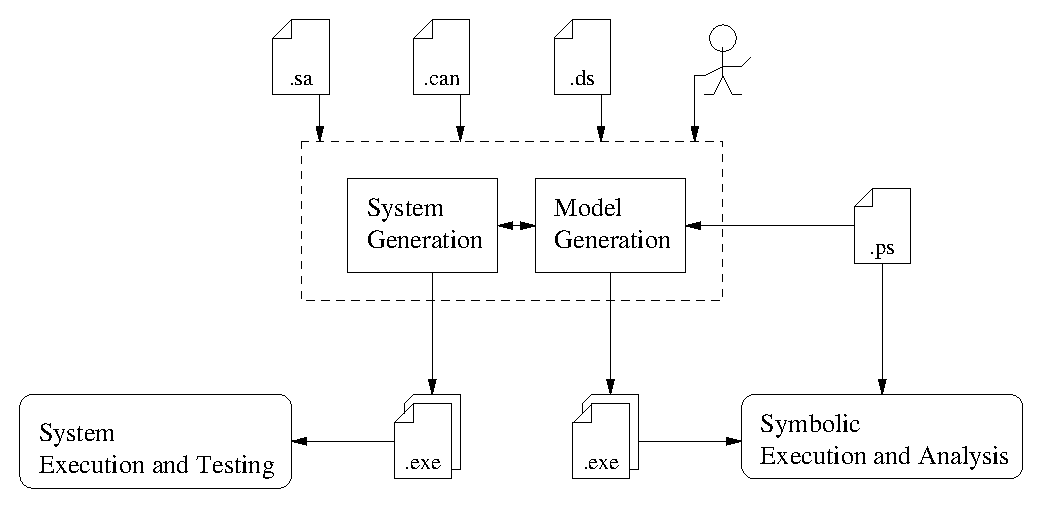
\includegraphics[width=.6\linewidth]{PRACTICE/candle1.eps}
\end{center}

\medskip

\begin{center}
\begin{tabular}{|>{\tt}c|p{.75\linewidth}|}
\hline

\includegraphics[width=.75cm]{PRACTICE/user.eps} & \raisebox{.5cm}{
\parbox[t]{\linewidth}{User commands for all tools are entered using a 
 graphical user interface to the development environment which checks 
 consistency.}} \\
.ds & Specification files for the data state and sequential operations 
      of each system process. Model-based specification languages such as B, Z
      or VDM can be used. Sequential code is developed from specifications
      using a standard methodology, e.g. refinement. Abstract data model
      is extracted from the same specifications for system verification.  \\
.can & \candle\ program modules: contain a description of the dynamic behaviour
  of processes including communication and synchronisation. Declare broadcast
  channels, including message identifiers and their priorities.\\
.sa & System architecture files: map processes to processors, communication
  channels to CAN buses, etc.;  describe the properties of system 
  components, e.g. processors, CAN buses and hardware timers in order to allow 
  the prediction of timing properties. \\
.ps & Property specification file: a specification of system
properties using a logic such as TCTL, a specification TA, or
a regular expression. Can be used by model generator to optimise model for 
verification of specific properties. \\
\hline
\end{tabular}
\end{center}
\end{minipage}
\caption{\candle\ Development Environment: Architecture\label{fig:prcandlearch}}
\end{figure}
It is intended that system implementation in \candle\ will follow 
a similar path to \esterel~\cite{ber:98b} and \aorta~\cite{bra:95}.
This will be the subject of a future research project and is 
not considered further here. The remainder of this section is devoted
to the model generation and analysis components of the validation
environment.


\subsection{Validation Environment}
The validation environment of \candle\ consists of components for
model generation and analysis. The core of the validation environment is
organised according to the principles of the \opencaesar\
architecture~\cite{gar:98}. This approach means that 
the CADP tool box~\cite{fgk:96} and 
\openkronos~\cite{tri:98} are immediately applicable to \candle\
programs; it also provides a very flexible mechanism for extending the
validation environment in the future.  The architecture of the
\candle\ validation environment is illustrated in
Figure~\ref{fig:prmodelgen}. 
\begin{figure}
\begin{minipage}{\textwidth}
\begin{center}
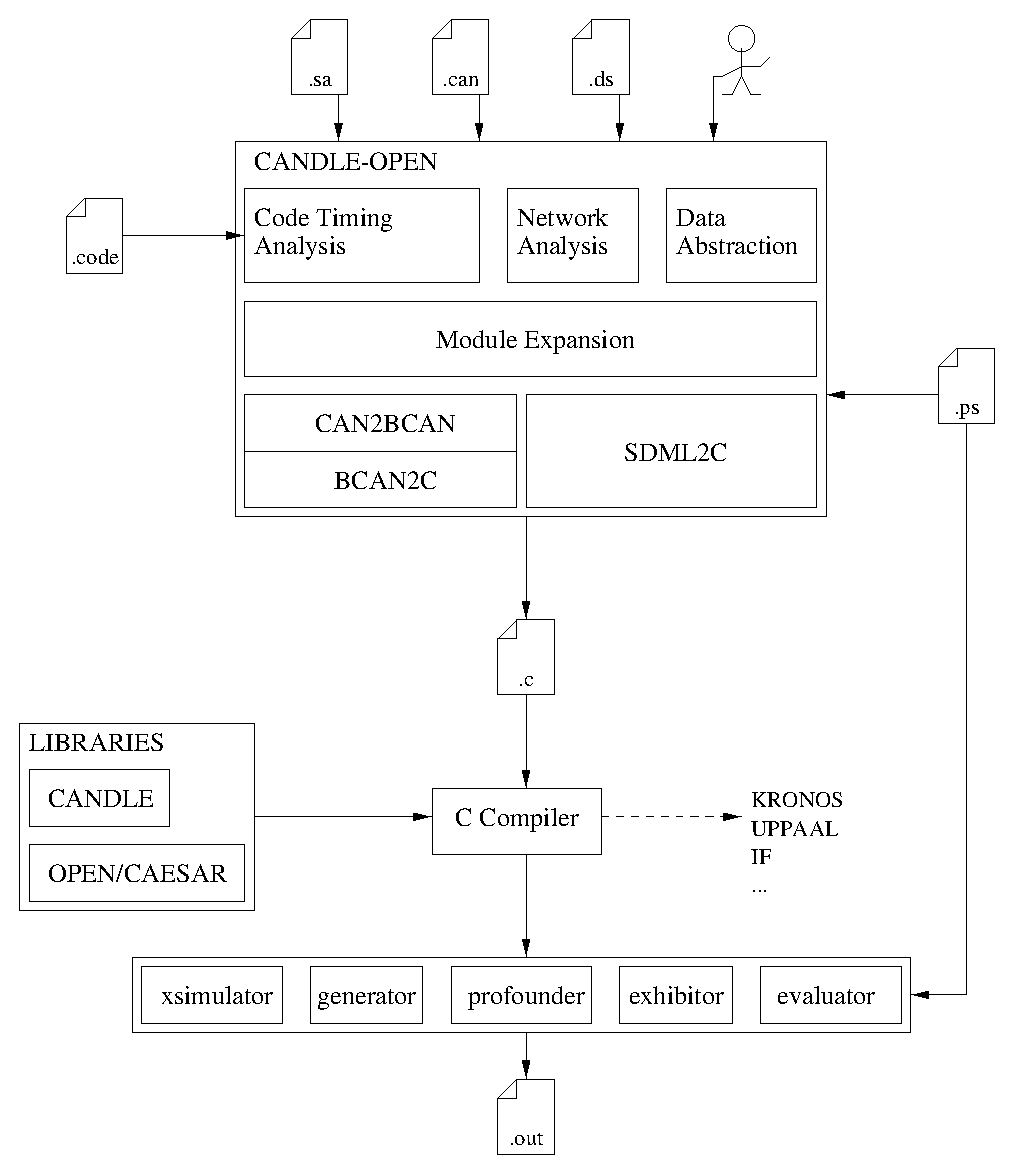
\includegraphics[width=.6\linewidth]{PRACTICE/candle2.eps}
\end{center}

\medskip
\begin{center}
\begin{tabular}{|>{\tt}c|p{.75\linewidth}|}
\hline
.code & Source and object code files of implemented system; produced by system generation component and required by model generation component for code 
timing analysis. \\
.c & Source code of the LTS module; combined with \candle\ and \opencaesar\
 libraries to produce executable analysis program. \\
.out & Output of symbolic analysis: Reachability graph, Yes/No answer, Timed/Untimed diagnostic trace etc. \\
\hline
\end{tabular}
\end{center}
\end{minipage}
\caption{\candle\ Validation Environment: Architecture\label{fig:prmodelgen}}
\end{figure}
Its main features are discussed in more detail below.

\subsection{The \opencaesar\ Architecture}
The design of the \opencaesar\ architecture evolved during the course
of projects to extend the functionality of the \caesar\
compiler~\cite{gar:92}, a translator from LOTOS programs to labelled
transition systems. Functional extensions included tools for random
execution, interactive simulation, behavioural equivalence checking,
temporal logic model-checking and test case generation. The desire to
allow these tools to be used with languages other than LOTOS led to a
design which encapsulates all language-dependent aspects.  The final
design offers a flexible and practical basis for the development of an
open, extensible validation environment.

Encapsulation of language dependencies is achieved in \opencaesar\ by
requiring that any source program is seen by the validation environment
as simply a labelled transition system which implements a well-defined
application programming interface (API). The LTS API provides access to
a representation of states and labels, and primitive operations to
compute the transition relation (i.e., the initial state and successors
of a given state). Knowledge of a source program by validation tools
is restricted to the LTS API, which is implemented by a C program
generated by an \opencaesar-\emph{compliant compiler} for the source
language. 
    
\subsection{Model Generation}
\candleopen\ is the \opencaesar-compliant compiler for 
\candle~(Figure~\ref{fig:prmodelgen}). It translates a \candle\
program into a C program which implements the \opencaesar\ LTS API,
generating the \candle\ program's simulation graph on demand. \candleopen\
defines interfaces which integrate a number of loosely coupled 
components. These components are described briefly below. 
\begin{itemize}
\item \textbf{Code Timing Analysis}: 
This component provides a connection to a program for calculating
execution time bounds on sequential code fragments.  This can be used
to obtain bounds for the data operations and expressions of the
\candle\ program by analysing their implementations. Access to the
source and object code files of the implementation is provided by the
system generation module~(Figure~\ref{fig:prcandlearch}). The process
map and processor models are given by the system architecture files. So
far, we have experimented with the use of the CINDERELLA code timing
analysis tool for 68000 micro-processors~\cite{lmw:95}. Other code
timing tools remain to be investigated.  

In the case that the implementation of some data operation is not
available for analysis, as will be the case quite often in the early
stages of a design, execution time bounds are obtained from the
\trm{bounds} clause of the \sdml\ model of the operation.  
The user can configure the development environment to obtain the
bounds on each data operation either by analysis of its
implementation, by examination of its \trm{bounds} clause, or by user
input via the keyboard. This allows the design to be explored in
whatever way is judged to be most convenient or interesting.

\item \textbf{Network Analysis}:
This component constructs the static network model, which defines
for each communication channel, its message set, message priorities and
message transmission latencies. The message set and message priorities
of each channel are stated explicitly in the \candle\ program. Calculation
of transmission latencies depends upon the characteristics of the
physical communication links implementing the channels and upon
the size of message packets. 

\item \textbf{Data Abstraction}:
This component constructs an abstract data model from a data specification.
The abstract data model is described in \sdml\ and currently is generated by 
the user. The integration into \candleopen\ of a tool such as 
InVeSt~\cite{blo:98} to support the construction of the abstract model is
envisaged.  

\item \textbf{Module Expansion}:
This component constructs a `flattened' \candle\ program by in-line
expansion of all module instantiations. 
\item \textbf{CAN2BCAN, BCAN2C, SDML2C}:
These components combine to generate the C program which implements the
LTS module. CAN2BCAN translates the flattened \candle\ program 
to its equivalent \bcandle\ representation, using the techniques
described in~\Sec\ref{sec:prtrans}. BCAN2C generates the C
functions to implement the algorithm described in~\Sec\ref{sec:sgonthefly} to
compute the transition relation of the simulation graph. SDML2C
generates C functions to implement the data operations and predicates.
As an alternative to generating code to construct the simulation graph
on-the-fly, the user can choose to construct a TA in KRONOS \trm{.tg} format, 
for later analysis. Although not yet implemented, other outputs which could 
be easily generated include UPPAAL \trm{.ta} format~\cite{lpy:97} and 
IF code~\cite{bfg:99}. These may give access to a wider range of
analyses and optimisations.  
\end{itemize}  
\subsubsection{Optimisation}
A variety of optimisations can be applied at several stages of the
model generation process, in order to combat state explosion. For
example, \emph{variable analysis}~\cite{bfg:99b,ss:98} can improve the
quality of C functions generated by BCAN2C and SDML2C, by identifying
dead variables which can be consistently reset. In addition, it seems
possible to take advantage of \emph{program slicing}
techniques~\cite{cdh:00,hdz:00,ls:98}, which can reduce the size of a
model by removing those parts of it which cannot affect the outcome of
the analysis of some specified property. Application of such 
optimisations remains to be investigated.

\subsection{Model Exploration}
A variety of tools can be applied to the exploration of generated LTS
models.  Many are provided by exploration modules from CADP or
\openkronos; the {\tt generator} module has been developed
specifically for \candle, in order to experiment with the MA state
storage technique described in Chapter~\ref{chap:sggen}.

\begin{itemize}
\item {\tt xsimulator} is an interactive simulator allowing step-by-step
  exploration of the simulation graph in a window-based environment.
\item {\tt evaluator} implements local and global algorithms for 
  on-the-fly model-checking of branching $\mu$-calculus.
\item {\tt exhibitor} performs a depth-first or breadth-first
  search  for a finite untimed trail matching an input regular expression. 
\item {\tt profounder} is an \openkronos\ module which implements
  an algorithm to test for language emptiness of the simulation graph
  and a specification TBA.
\item {\tt generator} builds the simulation graph of the system, using
  one of several user-specified state storage mechanisms.
\end{itemize}  


\section{An example\label{sec:prcanexample}}
In this section, we give an example of the use of \candle\ in
modelling a slightly larger control system. The example is a
modified version of the steam boiler control
problem~\cite{abl:96}. 

\subsection{The \candle\ program}
We consider a system comprising a steam boiler,
a pump, and a water-level sensor. We assume that the pump controls the
flow of water into the boiler and that steam is drawn off via a steam
outlet pipe. The water-level sensor gives the level of water in the
tank. The purpose of the control program is to ensure that the water
level is maintained within minimum and maximum bounds, or to shutdown
the system if failure of the water-level sensor is detected.
\begin{figure} 
\begin{center} 
\begin{minipage}{.5\linewidth}
\scriptsize 

\begin{verbatim} 
module Boiler is
   behaviour
     WaterLevel[Msecs(5)/WL_READY_PERIOD,
               Msecs(10)/WL_NORMAL_PERIOD, w1/w]
   | 
     Pump[Msecs(5)/PUMP_READY_PERIOD]
 
   | 
     Controller[Msecs(15)/SENSOR_TIMEDOUT, w2/w]
end module
\end{verbatim}
\end{minipage}
\end{center}
\caption{The Steam Boiler module\label{fig:prsteamboiler}}
\end{figure}

\begin{figure}
\begin{tabular}{l@{\hspace{.1\linewidth}}r}
\begin{minipage}{.4\linewidth}
\scriptsize
\begin{verbatim}  
module WaterLevel is
  const 
    WL_READY_PERIOD  : duration;
    WL_NORMAL_PERIOD : duration
  type 
    water_level
  procedure 
    InitSensor(out water_level);
    ReadSensor(out water_level)
  channel 
    k : (shutdown.unit, 
         level.water_level, 
         start.unit, 
         sensor_ready.unit)
  var
    w : water_level
  behaviour
    InitSensor(w);
    select
    :: rcv(k,start)
    in
      every WL_READY_PERIOD do
        snd(k,sensor_ready)
      end every
    end select;
    select
    :: rcv(k,shutdown) ; idle
    in
      every WL_NORMAL_PERIOD do
        ReadSensor(w);
        snd(k,level.w)      
      end every
    end select
end module 
\end{verbatim}
\end{minipage}
&
\begin{minipage}{.4\linewidth}
\scriptsize
\begin{verbatim}
module Pump is
  const
    PUMP_READY_PERIOD :  duration
  type
    pump_status
  procedure
    InitPump(out pump_status); 
    PumpOn(out pump_status); 
    PumpOff(out pump_status)
  channel
    k : (shutdown.unit, 
         pump_off.unit, 
         pump_on.unit,
         start.unit, 
         pump_ready.unit)
  var
    p : pump_status
  behaviour
    InitPump(p);
    select
    :: rcv(k,start)
    in
      every PUMP_READY_PERIOD do
        snd(k,pump_ready)
      end every  
    end select;
    select  
    :: rcv(k,shutdown); PumpOff(p); idle
    in
      loop do
        select
        :: rcv(k,pump_on) ; PumpOn(p)
        :: rcv(k,pump_off) ; PumpOff(p)
        end select
      end loop
    end select
end module      
\end{verbatim}
\end{minipage}
\\
\hfil \strut (a) \hfil & \hfil \strut (b) \hfil 
\end{tabular}
\caption{Water-level Sensor and Pump modules\label{fig:prsensorandpump}}
\end{figure}

\begin{figure}
\begin{center}
\begin{minipage}{.7\linewidth}
\scriptsize
\begin{verbatim}
module Controller is
  const 
    SENSOR_TIMEDOUT : duration
  type 
    water_level
  procedure
    InitController(out water_level)
  function
    IsHighLevel(water_level) : boolean;
    IsLowLevel(water_level)  : boolean
  channel 
    k : (shutdown.unit, pumpoff.unit, pumpon.unit,
         level.water_level, start.unit, pump_ready.unit,
         sensor_ready.unit)
  var 
    w : water_level
  behaviour
    InitController(w);
    select
    :: rcv(k,sensor_ready); rcv(k,pump_ready)
    :: rcv(k,pump_ready); rcv(k,sensor_ready)
    end select;
    snd(k,start);
    loop do
      select
      :: rcv(k,level.w);
         if    IsHighLevel(w) then snd(k,pump_off)
         elsif IsLowLevel(w)  then snd (k,pump_on)
         end if
      :: elapse SENSOR_TIMEDOUT; snd(k,shutdown); idle
      end select
    end loop
end module
\end{verbatim}
\end{minipage}
\end{center}
\caption{Controller module\label{fig:prcontroller}}
\end{figure}

\begin{figure}
\begin{center}
\begin{minipage}{.8\linewidth}
\scriptsize
\begin{verbatim}
data Boiler is
type water_level is {low, ok, high}
type pump_status is {on, off}

procedure 
  InitSensor(out wl : water_level) is bounds Cycles(300); Cycles(350)
    begin wl := ok end ;

  InitPump(out p : pump_status) is bounds Cycles(250); Cycles(1500)
    begin p := off end ;

  InitController(out wl : water_level) is bounds Cycles(400); Cycles(500) 
    begin wl := ok end;

  PumpOn(out p : pump_status) is bounds Cycles(200); Cycles(300)
    begin p := on end;

  PumpOff(out p : pump_status) is bounds Cycles(200); Cycles(300)
    begin p := off end 

  ReadSensor(out wl : water_level) is bounds Cycles(50); Cycles(75)
    begin wl := any water_level end

function 
  IsHighLevel(wl : water_level) : boolean is bounds Cycles(10); Cycles(15)
    begin return (wl = high) end;

  IsLowLevel(wl : water_level) : boolean is bounds Cycles(10); Cycles(15)
    begin return (wl = low) end
end data
\end{verbatim}
\end{minipage}
\end{center}
\caption{Steam Boiler Data Module\label{fig:prboilerdata}}
\end{figure}

The main program module is $Boiler$, shown in
Figure~\ref{fig:prsteamboiler}. It shows that the system is structured as the
parallel composition of three processes: $WaterLevel$, $Pump$ and
$Controller$, which are described in Figures~\ref{fig:prsensorandpump}
and~\ref{fig:prcontroller}. Figure~\ref{fig:prboilerdata} shows the
data module for the system.  

Each process executes three phases:
\emph{local initialisation}, \emph{ready} and \emph{normal}. 
\begin{itemize}
\item
In the local initialisation phase, a process resets its devices and
initialises its local data. It is assumed that the system is started
with the water level in the boiler between $low$ and $high$,
 and the pump $off$.
\item
In the ready phase, the $WaterLevel$ and $Pump$ processes repeatedly
transmit a $ready$ message until they receive a $start$ message from
the $Controller$. The $start$ message is broadcast by $Controller$
after it has received a $ready$ message from both $Waterlevel$ and
$Pump$.
\item
In normal operation, $WaterLevel$, repeatedly reads the water-level
sensor, updating a data variable with the current sensor value before
broadcasting the value on channel $k$. The $Controller$ process
receives the sensor value from channel $\kk$ and stores it in a data
variable. $IsLowLevel$ and $IsHighLevel$ are boolean functions on the
data state, used to test the value of the water level variable.  If
the level is too high, a message is sent to turn off the pump, if the
level is too low, a message is sent to turn on the pump, otherwise the
pump is left in its current state.  If $Controller$ does not receive a
water-level message before timing out, it is assumed that the water-level
sensor is faulty and a $shutdown$ message is broadcast which brings the
operation of the system to a halt with the pump turned off. We assume
that the system is then made safe manually.
\end{itemize}

\subsection{The \bcandle\ model}
The \candle\ program for the steam boiler can be translated into a
\bcandle\ model, as shown in Figure~\ref{fig:prbcboiler}. 

\begin{figure}
\begin{center}
\begin{minipage}{.6\linewidth}
\scriptsize
\begin{verbatim}
WaterLevel | Pump | Controller 

where

WaterLevel = [InitSensor: 300,350]; WL_Ready; WL_Normal
WL_Ready = WL_Ready0 [> k?start._
WL_Ready0 = k!sensor_ready._ ; idle 
            [> [WL_ReadyPeriod: 5000,5100] ; WL_Ready0
WL_Normal = (WL_Normal0 [> k?shutdown._ ; idle)
WL_Normal0 =
    [ReadWaterLevel:50,75]; k!level.w1 ; idle
    [>
    [WL_NormalPeriod:10000,10250]; WL_Normal0

Pump = [InitPump:250,1500]; P_Ready; P_Normal
P_Ready = P_Ready0 [> k?start._
P_Ready0 = k!pump_ready._ ; idle 
            [> [P_ReadyPeriod: 5000,5100] ; P_Ready0
P_Normal = (P_Normal0 [> k?shutdown._; [PumpOff:200,300] ; idle)
P_Normal0 = (k?pumpon._ ; [PumpOn:200,300] + 
             k?pumpoff._ ; [PumpOff:200,300]); 
            P_Normal0

Controller = [InitController:400,500]; C_Ready; C_Normal
C_Ready = (k?sensor_ready._ ; k?pump_ready._ + 
           k?pump_ready._ ; k?sensor_ready._);
           k!start._ 
C_Normal = k?level.w2;  
             [TestHighLevel: 10,15];
             (HighLevel -> k!pumpoff._ +
              notHighLevel -> 
                [TestLowLevel: 10,15];
                (LowLevel -> k!pumpon._ +
                 notLowLevel -> null));
             C_Normal 
           + 
           [SensorTimedOut: 15000,15500]; k!shutdown._ ; idle
    
network 
/*                  Pri   dlb  dub  dlB duB   */
k = (shutdown       : 1,   35,  43,  11, 13;
     pumpoff        : 2,   35,  43,  11, 13;
     pumpon         : 3,   35,  43,  11, 13;
     level          : 4,   43,  53,  11, 13;
     start          : 5,   35,  43,  11, 13;
     pump_ready     : 6,   35,  43,  11, 13;
     sensor_ready   : 7,   35,  43,  11, 13
     )
data w1, w2, p
\end{verbatim}
\end{minipage}
\end{center}
\caption{A \bcandle\ model for a simple boiler controller\label{fig:prbcboiler}}
\end{figure} 

We have made a number of simplifying assumptions in order to 
clarify the relationship between the program and its model:
\begin{itemize}
\item Each process is allocated to its own dedicated processor.
\item All processors run at the same speed, where $1$ clock cycle is
   assumed to be $1\mu$sec, which is assumed to be equivalent to $1$ unit of 
   \trm{duration}.
\item The bus implementing channel $\kk$ runs at $10^6 bit/s$, i.e.
  $1$ bit is transmitted in $1\mu$sec.
\item The bounds on all $pre\_snd$, $post\_snd$, $pre\_rcv$ and $post\_rcv$
  operations are $0$, and so these operations have been omitted from the 
  model.  
\end{itemize} 

The description of process behaviour in Figure~\ref{fig:prbcboiler} has been 
derived using the translation method described earlier, with the assumptions
stated above and with some small modifications to aid readability: recursion
is expressed using the equational style, rather than by using explicit
$\rec$ terms; `extra' equational definitions have been introduced to 
emphasise the initialisation, ready and normal phases of process behaviour.

The network section of the model is derived from the \candle\
\trm{channel} declarations and the assumptions about the underlying
communication mechanism. It defines the network structure -- in this
case, simply a single channel -- giving the priority of messages and
the transmission latency function. Notice that all messages, except
$level$ messages, consist only of a message identifier, whereas
$level$ messages contain a water level value in addition to the
message identifier, and hence have a greater pre-acceptance latency.

The data section declares the names of the data variables used in the model. 
The \bcandle\ data environment is constructed from the \sdml\ data module
in a straightforward way, as described in~\Sec\ref{ss:prcantransexample}.
We do not elaborate the data environment here.

\subsection{Analysis of the model}\label{ss:prexampleanal}
The \candleopen\ environment can be used to generate the simulation graph
of the \bcandle\ model, and to explore it interactively, or exhaustively, to
ensure that it exhibits desirable behaviour. In this case, \trm{generator}
produces the graph in less than a second on a 233MHz Pentium II, running 
RedHat Linux 5.2. The output
\begin{flushleft}
\begin{minipage}{\textwidth} 
\begin{verbatim}
      generator: Release 1.1.1 Thu Oct 27 22:03:15 GMT 2000
      Simulation Graph: Boiler
      #states                   1963
      #trans                    2661
      #matrices                 1123
\end{verbatim} 
\end{minipage}
\end{flushleft}
shows the number of states and transitions in the simulation graph. The
number of matrices indicates the number of distinct clock zones explored.
It is worth noting that the simulation graph for the boiler control
system is very much smaller than the equivalent TA generated from the
\bcandle\ model using the standard techniques of Chapter~\ref{chap:tggen}.
That TA has more than 500,000 locations, exceeding the capacity of 
model checkers such as KRONOS. This is a clear indication of the benefit
of generating the simulation graph `on-the-fly'. The application
of clock activity reduction to the example reduces the number of clocks
required from 12 to 5. This also has a significant effect on the size of
the model, reducing the number of states in the simulation graph from
$>115,000$ to $1963$.
 
The simulation graph can be checked for a variety of properties, which
increase confidence in the correctness of the control system. A number
of simple properties, which the graph satisfies, are discussed below.
\begin{notation}
Notice that the properties are expressed using predicates over the state
variables, rather than using a propositional encoding as required by KRONOS.
The status and pending message queue of a channel $\kk$ are denoted
$\kk.status$ and $\kk.queue$, respectively. See \Sec\ref{ss:bcnetstructure}
for an explanation of other channel notation.
\end{notation}  
\begin{enumerate}
\item Basic `sanity' checks:  
  \begin{enumerate}
    \item The model is non-Zeno. \\
          \hspace*{2em}$init \implies \aalways{}\eeventually{=1} \true$
    \item Whenever the channel
      is not busy, and there are messages pending transmission, the channel
      begins transmitting a message immediately. \\
          \hspace*{2em} $\aalways{}((\kk.status = \FREE \land \kk.queue \neq \emq) 
            \implies \aeventually{=0} \kk.status = \PRE)$
  \end{enumerate}
  In fact, it can be shown that any persistent \bcandle\ model satisfies
  these properties. However, failure to satisfy either property alerts the 
  user to a fundamental error in the construction of the model.
\item Properties of the communication system:
  \begin{enumerate} 
    \item A pending message is never overwritten, i.e. once a message
      is queued, it will be transmitted before another message with the
      same identifier is queued. \\ 
      \hspace*{2em}
      $\aalways{}(\enable(\kk!\ii.\_) \implies \forall \jj \in
      \dom(\kk.queue) \such \kk.queue[\jj] \neq \ii.\_)$
    \item When any message transmission reaches the acceptance point,
      some process will be able to accept the message. \\ 
      \hspace*{2em}
      $\aalways{}(\enable(\kk\offers\mm) \implies
      \aeventually{=0}\enable(\kk?\mm))$
    \item The time between acceptance tests for any type of message is at 
      least $\ti$. \\ 
      \hspace*{2em} 
      $\aalways{}(\enable(\kk\offers\ii.\_) \implies 
      \aeventually{=0}(\aalways{<\ti} \lnot \enable(\kk\offers\ii.\_)))$ 
  \end{enumerate} 
    Of course, there are many systems for which these properties are
    not required. But, very often, the failure of one or more of them
    is an indication of a flaw in the implementation of the
    control system.  For example, property (c) is helpful in checking
    the behaviour of a multi-tasking node implemented with round robin
    scheduling and polled communication, as the value of $\ti$ for any
    channel and message type should not be less than the quantum of
    the scheduler, otherwise messages may be lost.
\item Basic response properties:
  \begin{enumerate}
    \item If a $low$ water level is detected, then the pump
      will be $on$ within $1$msec. \\
            \hspace*{2em} $\aalways{}(w1 = low \implies  
                   \aeventually{\leq 1000}(p = on))$
    \item If a $high$ water level is detected, then the pump will be $off$ 
      within $1$msec. \\
            \hspace*{2em} $\aalways{}(w1 = high \implies 
                   \aeventually{\leq 1000}(p = off))$
  \end{enumerate}
\item Further response properties:
  \begin{enumerate}
    \item If it is not possible for the $Controller$ to receive a $level$ 
      message immediately, then, within $16$msecs, it can receive such
      a message, or it will transmit the $shutdown$ message. \\ 
           \hspace*{2em} $\aalways{}(\lnot \enable(\kk?level.\_) \implies$ \\ 
           \hspace*{2cm} $\aeventually{\leq 16000}(\enable(\kk?level.\_) \lor 
                                     \enable(\kk!shutdown)))$
    \item If transmission of the $shutdown$ message is enabled, then,
       within $1$msec, the pump is turned $off$ and the system idles. \\
            \hspace*{2em} $\aalways{}(\enable(\kk!shutdown) \implies 
            \aeventually{\leq 1000}(p = off \land 
                         \aalways{}(\lnot \enable(\_))))$
  \end{enumerate}
\end{enumerate}

Verification of some control system properties is most conveniently
undertaken by an analysis of the control system model in conjunction
with a model of its environment.  For example, to verify that the
boiler control system always maintains the level of water within
acceptable bounds, a model of the boiler can be constructed, 
including aspects of its behaviour such as: the rate of flow of water
from the pump; the response lag of the pump to a control command; the
rate of flow of steam from the boiler, and so on.  
Henzinger and Wong-Toi~\cite{hw:96} describe a
hybrid automata model of a steam boiler, which could form the basis of a 
suitable environmental model for composition with our model of the boiler
control system. As usual, the limiting factor is the state
explosion problem. A benefit of our approach is that it is possible to take
advantage of a minimisation tool, such as \minim~\cite{tri:98}, in order
to reduce the size of the control system model before composing it
with an environmental model.

\section{Conclusions and Related Work\label{sec:prconc}}
\subsection{Conclusions}
We have defined a programming language for broadcasting embedded
control systems. The language has many of the constructs which one
would expect in a modern, real-time language~\cite{bw:01}, and it has
been shown that the process language \bcandle\ is expressive enough to
give a semantics to these constructs in a natural way. We have
described a development and validation environment which integrates a
variety of languages and tools.  In particular, the environment
supports the translation of \candle\ programs to TA, enabling the
application of tools such as KRONOS and CADP for validation. Future
work will include further development of the language, in particular
to improve the module system, and also further development of the tool
support. Automation of the development of executable abstract data
models from B or VDM specifications is also of interest. An important
focus of future work will be the efficient composition of control
system models with environmental models in order to allow validation
of a wider range of system properties. Finally, more experience is
needed of applying both language and tools to a wider range of case
studies, so that the techniques can be tested on examples which are
more realistic in terms of their size and complexity than those which
are described in this chapter.

\subsection{Related Work}
\esterel~\cite{bg:92} is the classical example of a language which
supports both the development and validation of embedded systems.  It
represents the synchronous approach which has been so effective in the
uniprocessor domain. Interest in the application of model-checking to
asynchronous systems is comparatively recent. One of the first tools
for untimed systems is VeriSoft~\cite{god:97} which supports stateless
search in the verification of C programs. Holzmann and
Smith~\cite{hs:99} describe an approach in which a SPIN~\cite{hol:97}
model is extracted from an annotated C program, allowing the checking
of properties specified in LTL.  Related approaches to the
verification of Java programs are described by Havelund and
Pressburger~\cite{hp:00} and Corbett~et~al.~\cite{cdh:00}.  The
latter work builds upon experience gained in applying similar
techniques to the verification of Ada programs~\cite{dpc:98}.
Huch~\cite{huc:99} has developed a dedicated model checker for a
subset of Erlang -- an untyped higher-order concurrent functional
language with asynchronous communication primitives. All of these
approaches employ techniques to construct an abstract model using only
the source code of the program to be verified. Our approach enforces a
clear separation of control algorithms and sequential data operations,
and assumes that abstract specifications are available for the latter.
We believe that these specifications will prove to be a better
starting point for the construction of efficient models.

In the case of timed systems, the work of Corbett~\cite{cor:96} is the
most ambitious in its choice of input language.  He describes a method
for translating (a subset of) Ada programs into hybrid automata, so
enabling the checking of a variety of temporal properties using the
HyTech~\cite{hhw:97} model checker. His models can accommodate fixed
priority pre-emptive scheduling of concurrent tasks but he considers
only uniprocessor systems, deferring distributed systems to further
work. Hune~\cite{hun:99} considers the problem of using
UPPAAL~\cite{lpy:97} for verifying programs executing on the LEGO RCX
brick. The LEGO RCX brick is part of the LEGO MINDSTORMS range of LEGO
toys. It contains a micro-processor and is equipped with three
sensors, three actuators and an infra-red port for communication to
enable program downloading.  Hune describes a translation from the RCX
assembly language into a network of TA described using the UPPAAL
input language. Again, the work is restricted to uniprocessor systems;
the scheduling policy is round-robin.  Iversen~et~al.~\cite{ikl:00}
also consider the same problem, but allow the use of a more expressive
programming language, NQC (Not Quite C), which is a restricted form of
C. Dierks~\cite{die:01} introduces PLC-automata with a view to
developing and analysing real-time systems implemented with
programmable logic controllers. He describes a method for translating
PLC-automata to timed automata so that KRONOS and UPPAAL can be used
for the analysis. 

This brief survey of related work is evidence of the recent interest
in applying model-checking to the analysis of embedded system
implementations. We believe that the work described in this chapter is
the first to present a general method for real-time model-checking of
distributed, high-level programs implemented on an industry-standard,
broadcast network.

